\documentclass[12pt,a4paper]{book} % ou article, memoir, report, etc.

%usepackage permet d'utiliser un module complémentaire.

% Marges, retraits et espacement
\usepackage[margin=2.5cm]{geometry}
%espacement des lignes
\usepackage{setspace}
\onehalfspacing
\setlength\parindent{1cm}

\usepackage{tocbibind}

\usepackage[colorlinks=true]{hyperref}

%Le package Babel permet de gérer différentes normes linguistiques et typographiques
\usepackage[english,italian,french]{babel}


%Nouvelle syntaxe ici: une commande avec une option entre []
\usepackage[utf8]{inputenc}

%Gérer l'encodage des caractères en sortie
\usepackage[T1]{fontenc}
\usepackage[final]{pdfpages}
%Changer la fonte de caractère
\usepackage{newcent}
%\usepackage{lmodern}
%\usepackage{charter}
%Pour les maniaques du Times \usepackage{txfonts}
%Palatino \usepackage{mathpazo}

%Métadonnées du document
%Auteur
\author{Josselin Morvan}
\title{}
%La commande date est optionnelle
%\date{2 janvier 1950}
\date{Version du \today}


%Écrire les mots inconnus du dictionnaire pour la césure/l'hyphénation
%\hyphenation{Ajou-t-ons}


%Autres modules complémentaires
\usepackage{lettrine}
%\usepackage[pdftex]{graphicx}

%pour le mode paysage je dois utiliser deux packages
%\usepackage{lscape}%pour le mode paysage
%\usepackage{pdflscape}%pour l'indiquer dans les métadonnées du pdf.

%pour le dessin
\usepackage{tikz}%pour le dessin
\usepackage{tikz-qtree}%pour les arbres 

\usepackage{caption}%pour ne pas numéroter les figures (on ajoute une étoile après caption)

%pour créer un Index
\usepackage{makeidx}
%pour activer la création de l'index.
\makeindex 

%Appeller le package pour les bibliographies
\usepackage[backend=biber, sorting=nyt, style=ENC]{biblatex}
%appel de la ressource bibliographique.
\addbibresource{memoire.bib}
%pour les guillemets
\usepackage[babel]{csquotes}

% personnalisation pour la citation de code.
\usepackage{listingsutf8}

\usepackage{color}

\lstset{
  basicstyle=\footnotesize,
  frame=single,
  columns=fullflexible,
  showstringspaces=false,
  breaklines        = true,
  breakatwhitespace = true,
  %breakindent       = 2ex,
  escapechar        = *,
  commentstyle=\color{gray}\upshape
}

\definecolor{maroon}{rgb}{0.5,0,0}
\definecolor{mygray}{rgb}{0.5,0.5,0.5}
\definecolor{darkgreen}{rgb}{0,0.5,0}
\definecolor{fondcode}{rgb}{0.95,0.95,0.95}
\lstdefinelanguage{XML}
{
  basicstyle=\footnotesize,
  morestring=[s]{"}{"},
  morecomment=[s]{?}{?},
  morecomment=[s]{!--}{--},
  commentstyle=\color{darkgreen},
  moredelim=[s][\color{black}]{>}{<},
  moredelim=[s][\color{orange}]{\ }{=},
  stringstyle=\color{maroon},
  identifierstyle=\color{blue}
}
\lstset{literate=
  {á}{{\'a}}1 {é}{{\'e}}1 {í}{{\'i}}1 {ó}{{\'o}}1 {ú}{{\'u}}1
  {Á}{{\'A}}1 {É}{{\'E}}1 {Í}{{\'I}}1 {Ó}{{\'O}}1 {Ú}{{\'U}}1
  {à}{{\`a}}1 {è}{{\`e}}1 {ì}{{\`i}}1 {ò}{{\`o}}1 {ù}{{\`u}}1
  {À}{{\`A}}1 {È}{{\'E}}1 {Ì}{{\`I}}1 {Ò}{{\`O}}1 {Ù}{{\`U}}1
  {ä}{{\"a}}1 {ë}{{\"e}}1 {ï}{{\"i}}1 {ö}{{\"o}}1 {ü}{{\"u}}1
  {Ä}{{\"A}}1 {Ë}{{\"E}}1 {Ï}{{\"I}}1 {Ö}{{\"O}}1 {Ü}{{\"U}}1
  {â}{{\^a}}1 {ê}{{\^e}}1 {î}{{\^i}}1 {ô}{{\^o}}1 {û}{{\^u}}1
  {Â}{{\^A}}1 {Ê}{{\^E}}1 {Î}{{\^I}}1 {Ô}{{\^O}}1 {Û}{{\^U}}1
  {œ}{{\oe}}1 {Œ}{{\OE}}1 {æ}{{\ae}}1 {Æ}{{\AE}}1 {ß}{{\ss}}1
  {ű}{{\H{u}}}1 {Ű}{{\H{U}}}1 {ő}{{\H{o}}}1 {Ő}{{\H{O}}}1
  {ç}{{\c c}}1 {Ç}{{\c C}}1 {ø}{{\o}}1 {å}{{\r a}}1 {Å}{{\r A}}1
  {€}{{\EUR}}1 {£}{{\pounds}}1
}
\definecolor{lightgrey}{rgb}{0.9,0.9,0.9}
\definecolor{darkgreen}{rgb}{0,0.6,0}
\lstset{language=XML}
\begin{document}

%\begin{abstract}

\frontmatter

\begin{titlepage}
\begin{center}

\bigskip

\begin{large}
\'ECOLE NATIONALE DES CHARTES
\end{large}
\begin{center}\rule{2cm}{0.02cm}\end{center}

\bigskip
\bigskip
\bigskip
\begin{Large}
\textbf{Josselin Morvan}\\
\end{Large}
\begin{normalsize} \textit{licencié en droit}\\
\textit{licencié en histoire de l'art}\\
\end{normalsize}

\bigskip
\bigskip
\bigskip

\begin{Huge}
\textbf{Modélisation XML-TEI, XSLT et publication web}\\

\end{Huge}
\bigskip
\bigskip
\begin{LARGE}
\textbf{La correspondance d'Armand Horel, un marin durant la Grande Guerre}\\
\end{LARGE}

\bigskip
\bigskip
\bigskip
\begin{large}
\end{large}
\vfill

\begin{large}
Mémoire pour le diplôme de master \\
\og Technologies numériques appliquées à l'histoire \fg{} \\
\bigskip
2015
\end{large}

\end{center}
\end{titlepage}

\thispagestyle{empty}

\cleardoublepage


\section*{Résumé}
\addcontentsline{toc}{chapter}{Résumé}
\bigskip

Ce mémoire a été réalisé à la suite d'un stage de trois mois et demi effectué à la bibliothèque de documentation internationale contemporaine (BDIC). Cet établissement spécialisé dans l'histoire du \begin{scriptsize}XX\end{scriptsize}\ieme{} et \begin{scriptsize}XXI\end{scriptsize}\ieme{} siècles, est impliqué depuis sa création dans le développement de nouveaux champs de recherches. À la fois bibliothèque, centre d'archives et musée, elle ne cherche pas seulement à mettre en lumière des documents inexploités, mais à impulser une nouvelle réflexion quant à leur exploitation, afin de faire émerger de nouvelles problématiques. La BDIC a depuis quelques années intégré l'aspect numérique dans sa démarche, en s'engageant aux côtés de la Maison de l'archéologie et de l'ethnologie (MAE), dans le Labex, \textit{les passés dans le présent} qui s'\og attache plus spécifiquement à comprendre les médiations de l'histoire à l'ère du numérique, les politiques de la mémoire et les appropriations sociales du passé en amont et en aval des politiques patrimoniales\fg{}.

\og Bibliothèque de et pour la recherche \fg{}, la BDIC est soucieuse d'accompagner ses usagers dans leurs prospections, en leur offrant notamment des outils qu'ils pourront mettre à profit dans leurs travaux. Le contexte de commémoration du centenaire de la Grande Guerre et l'intérêt grandissant du public pour les ressources liées au conflit, étaient propices au développement d'un modèle d'édition électronique en XML-TEI dédié aux correspondances. Cette modélisation a été réalisée avec comme objectifs principaux, de respecter les \og sources \fg{} au maximum lors de l'encodage, de proposer une version normalisée du texte et de permettre un double accès chrono-géographique aux documents. Ce modèle XML-TEI est accompagné d'une solution de publication web, mise en place à partir de feuilles de transformation XSL de deux types ; XML vers HTML pour la publication des lettres et XML vers XML pour une utilisation comme base de données de certaines informations. La correspondance d'Armand Horel, conservée à la BDIC, a permis de mettre en œuvre ces solutions d'édition et de publication électroniques. Le développement d'un site internet spécifique à ce fonds a nécessité l'écriture de feuilles de style CSS et de scripts JavaScript liés à la mise en forme et à l'ergonomie des pages web. 

\bigskip

\textbf{Mots-clés:} XML ; TEI ; XSLT ; édition électronique ; publication électronique ; correspondance ; géolocalisation.

\textbf{Informations bibliographiques:} Josselin Morvan, \textit{Modélisation XML-TEI, XSLT et publication web : La correspondance d'Armand Horel, un marin durant la Grande Guerre}, mémoire de master \og Technologies numériques appliquées à l'histoire \fg{}, dir. [Frédérique Joannic-Seta], École nationale des chartes, 2015.

\textbf{Avertissement:} ce mémoire est accompagné d'un appendice numérique consultable à l'adresse suivante : \url{github.com/sardinecan/TEIcorrespondances_horel}



\clearpage
\thispagestyle{empty}
\cleardoublepage



\section*{Remerciements}
\addcontentsline{toc}{chapter}{Remerciements}

\lettrine{L}{a réalisation de ce mémoire} a été possible grâce au concours de plusieurs personnes à qui je souhaiterais témoigner ma reconnaissance.
\bigskip

Tout d'abord, je voudrais adresser toute ma gratitude à ma directrice de stage, Frédérique Joannic-Seta, directrice adjointe de la BDIC, pour avoir rendu ce stage possible et pour m'avoir encouragé à formuler des propositions tout au long de cette entreprise. %todo travail sur les sources

J'aimerais également remercier Jean-Baptiste Camps, tuteur pédagogique et responsable du master \og technologies numériques appliquées à l'histoire \fg{} pour son enseignement et ses conseils avisés à propos du langage XML.

Je me dois également de remercier Emmanuel Chateau qui, le premier, m'a apporté son soutien et orienté vers les humanités numériques. Puis, que Camille Desenclos, Patrick Latour et Lionel Maurel acceptent ici ma gratitude pour leur soutien et leurs précieux conseils.

Enfin, que mes parents et amis acceptent ici mes remerciements pour leur support moral, intellectuel et leur écoute tout au long de ma démarche. Sans oublier Sara à qui je dois tant, pour sa confiance, sa patience et son soutien inestimable.

\clearpage
\thispagestyle{empty}
\cleardoublepage

\chapter*{Introduction}
\addcontentsline{toc}{chapter}{Introduction}

La bibliothèque de documentation internationale contemporaine (BDIC) est un établissement spécialisé dans l'histoire contemporaine et les relations internationales des \begin{scriptsize}XX\end{scriptsize}\ieme{} et \begin{scriptsize}XXI\end{scriptsize}\ieme{} siècle. À la fois bibliothèque, centre d'archives et musée, elle a été créée en janvier 1918 à  l'initiative d'un couple d'industriels, les époux Leblanc. Ce couple  décida de récolter dès le début de la guerre, tous les documents qui leur permettraient de comprendre les origines du conflit mondial. Elle se définit depuis toujours comme une \og bibliothèque de l'événement \fg{}\footcite{domenach_reflexion_1998}, dont la vocation est de collecter tous les matériaux pouvant servir à l'interprétation et l'écriture de l'histoire contemporaine.

\section*{\og Un laboratoire de et pour la recherche \fg{}\footcite{tesniere_laboratoire_2015}}

Depuis sa création, la bibliothèque de documentation internationale contemporaine s'est vue attribuer la double mission d'être à la fois \og une œuvre d'éducation populaire ---~et de diffusion des résultats de la recherche~--- \fg{} et un \og laboratoire d'histoire fondé sur les méthodes de l'érudition scientifique \fg{}\footcite{_recherche_????}. Elle a su apporter un regard neuf sur les fondements  des sources de l'histoire. Elle a intégré dans ses collections, des documents écrits et iconographiques qui étaient encore ignorés par les chercheurs. Cette réflexion des historiens révèle la cohabitation dans ses fonds, de sources primaires et secondaires.

Acteur de la recherche, la BDIC a pris conscience des enjeux du numérique en s'engageant notamment dans le Labex \textit{les passés dans le présent} dont elle est un des piliers avec la Maison de l'archéologie et de l'ethnologie (MAE). Ce laboratoire d'excellence s'attache \og à comprendre les médiations de l'histoire à l'ère du numérique, les politiques de la mémoire et les appropriations sociales du passé en amont et en aval des politiques patrimoniales \fg{}\footcite{_les_????}. Pôle associé de la Bibliothèque nationale de France, elle mène également une importante politique de numérisation de ses collections patrimoniales.

\section*{Un projet d'édition électronique de correspondances}

Attachée à sa mission d'accompagnement des chercheurs, la BDIC est soucieuse de leur proposer des outils qu'ils pourront mettre à profit dans leur travaux. Avec plus de soixante mille documents numérisés, sa bibliothèque numérique est l'une des plus importantes de l'enseignement supérieur\footnote{Bibliothèque numérique Argonnaute : \url{http://argonnaute.u-paris10.fr/}}. Ce type d'infrastructure représente un véritable bond en avant pour la recherche, particulièrement lorsqu'à l'instar de la BDIC,  les institutions patrimoniales décident d'offrir leurs documents sous licence ouverte.

Poursuivant cette démarche, la bibliothèque de documentation internationale contemporaine a souhaité se doter d'un modèle d'édition en XML-TEI dédié aux correspondances de poilus. Les ensembles épistolaires sont des sources importantes, demeurées paradoxalement, peu ou mal mises en valeur. Si elles sont susceptibles d'intéresser un grand nombre de chercheurs dans des domaines variés ---~histoire, philologie, biographie, linguistique etc.~--- il est dommage de constater qu'elles sont encore trop souvent reléguées à un rôle documentaire de second plan et non exploitées comme les sources primaires qu'elles représentent\footcite{vanhoutte_describing_2009}. En effet, ces matériaux ne sont pas toujours des plus aisés à manipuler ; ensembles hétérogènes, 
\begin{quote}
\begin{otherlanguage}{english}
They are produced by (at least) two people, writing in different locations, and contain a wealth of information of various kinds.
\end{otherlanguage}
\end{quote}
\begin{quote}
[i]ls sont produits par (au moins) deux personnes, communiquant depuis des lieux différents, et recelant une richesse d'information de différentes sortes\footcite{desenclos_early_2015}.
\end{quote}
Une édition de correspondances bien menée offre au plus grand nombre, des matériaux fiables, replacés dans leur contexte et qui pourront être facilement réexploités\footcite{nougaret_ledition_2015}. C'est là le principal enjeu auquel devait répondre ce stage ; mettre en place une modélisation XML-TEI simple, permettant à des personnes non spécialistes des nouvelles technologies ---~mais souhaitant toutefois les intégrer à leurs travaux~---, d'encoder un corpus de correspondances de manière à ce qu'il soit valorisable, dans leur approche, mais aussi réutilisable par d'autres, s'ils décident de le partager.  

Le projet a été élaboré autour de l'édition électronique de la correspondance d'Armand Horel\footnote{Bibliothèque de documentation internationale contemporaine ; F $\Delta$ 1854/20, Don de Madame la Comtesse de la Forest, [disponible en ligne : \url{http://argonnaute.u-paris10.fr/resource/a011403267952LEa5xJ}].}. Il a impliqué trois phases de développement : l'analyse du corpus afin de réaliser un modèle d'édition, la transcription et l'encodage d'une partie des lettres, et enfin, la réalisation d'une interface de publication électronique.



\clearpage
\thispagestyle{empty}
\cleardoublepage
\nocite{*}
\printbibliography

\mainmatter


\part{Éditer une correspondance de poilus}


\chapter{Mettre en valeur des sources}
La vocation de ce stage ne résidait pas tant dans l'édition de la correspondance d'Armand Horel, Quartier-maitre canonnier pendant la Grande Guerre, que d'offrir à la bibliothèque de documentation internationale contemporaine un modèle d'édition électronique. Celui-ci est destiné à la diffusion auprès d'usagers souhaitant intégrer le numérique à leur démarche. 
Toutefois, une modélisation nécessite de procéder à une analyse fine des matériaux afin de proposer des solutions cohérentes au regard des objectifs et principes éditoriaux retenus pour un tel projet. Une édition électronique est donc avant tout une édition. Il est important d'avoir cet élément en tête car si la mise en œuvre peut être différente ---~ne serait-ce que par le support d'édition proposé~—--, la démarche doit rester la même. Éditer, demande du temps et des moyens ; afin de rationaliser ces ressources, il est nécessaire de bien s'interroger sur les motivations de l'édition car elles guideront les différentes orientations du projet.

\section{L'édition de correspondances}
\subsection{Délimitation d'un corpus}
Pour un tel projet, la première question qui vient à l'esprit est de déterminer ce que l'on va éditer. Dans le cadre de ce stage, si le type des documents ciblés a été défini assez rapidement, il restait encore à qualifier un fonds qui puisse être l'objet de ce travail. Outre les intérêts historiques et techniques que nous développerons plus en détail par la suite, il a été retenu la correspondance d'Armand Horel, avec ses  cent cinquante cartes postales, qui était suffisamment consistante pour donner lieu à un premier projet d'édition. Comme nous l'avons vu plus haut, éditer est chronophage et demande des ressources. Cela nécessite de bien fixer à l'avance les limites de l'ensemble à traiter sous peine de ne pouvoir mener à bien  l'entreprise. Sur ce point, le numérique offre sans doute une plus grande souplesse dans la gestion du projet, dans la mesure où le versement des textes édités peut se repartir plus facilement dans le temps ; une édition papier aurait peut être contraint au choix d'une édition partielle. Sur cette question l'objectif du stage n'était pas d'encoder l'intégralité de la correspondance mais environ trente pour cent du corpus. Cela semble peu mais, outre la modélisation, il fallait également développer une interface de consultation en ligne, permettant de mettre en valeur les apports de l'édition numérique ainsi que la documentation attenante au modèle d'encodage. Au final, ce sont près de cent deux cartes postales et enveloppes qui ont été traitées.

Pour une édition de correspondances, les problématiques liées à la taille du corpus ne sont pas les seules à émerger. En effet, les ensembles épistolaires sont issus d'un processus d'échange entre ---~au moins~--- deux personnes communiquant sur des sujets variés depuis des lieux et à des dates différents. Une correspondance est un phénomène qui se développe et évolue dans le temps. Elle peut également être suivie ou discontinue et  impliquer plusieurs personnes. De plus, elle peut nous arriver lacunaire. Tous ces paramètres sont à prendre en compte dans la constitution du corpus, afin de construire un propos cohérent et quelque soit la manière dont ils s'imposent à nous, ils doivent être justifiés\footcite{desenclos_early_2015}. Enfin, le choix de ces documents doit être réfléchi et non le fruit du hasard ou par dépit, constituant ainsi un ensemble cohérent, avec l'intention de fournir au chercheur un outil fiable.


\subsection{Mettre en valeur des sources}
Pourquoi édite-t-on ? cette question doit être conservée à l'esprit durant tout le développement du projet.  Il ne s'agit pas encore de cibler un  type d'utilisateur ou quelle forme d'édition, nous souhaitons mettre en place.
%il est necessaire de determiner des objectifs auxquels toute edition scientifique doit répondre.
Il est ici question des objectifs auxquels toute édition scientifique doit répondre. 
En plus de diffuser ses textes auprès du plus large public possible, un éditeur scientifique doit également proposer des sources fiables et réutilisables pour la recherche\footcite[p. 19]{nougaret_ledition_2015}. Il doit aussi s'efforcer de rendre compréhensible le texte édité en le replaçant dans son contexte afin de reconstituer le propos des auteurs. Ainsi il cherchera par exemple à rassembler des recueils éparpillés, ou à combler les manques ; il est bien sûr, invraisemblable de restaurer un vide, mais il est souvent envisageable de créer des liens entre différents documents afin de compenser cette perte\footcite{desenclos_early_2015}\footcite[p. 19]{nougaret_ledition_2015}. Enfin, l'éditeur joue aussi un rôle dans la valorisation des sources. C'est intrinsèquement lié à son objectif de diffusion, qui doit favoriser l'accessibilité du public à ces matériaux, que l'éditeur participe à la mise en valeur de ces documents soit, en proposant des documents inédits, encore ignorés des chercheurs ou en participant à la protection des sources. Ces dernières une fois éditées et réceptibles, pouvant être retirées de la communication\footcite{nougaret_ledition_2015}.

Sur ce point de l'accès aux sources, le numérique joue indéniablement un grand rôle dans la mesure où toute édition publiée sur le web est abordable partout et par tous. Il faut toutefois bien faire la distinction entre la publication de fac-similé, comme le proposent certaines bibliothèques --- telle la BDIC --- et l'édition de textes; toutes deux répondent à des impératifs relativement différents. Malgré tout, ces démarches doivent être encouragées.
%todo développer ce point ? 

\section{Quel type d'édition}

\subsection{Définir une édition}
Qu'elle soit électronique ou papier, une édition constitue immanquablement une vue réduite de la source originale et en conséquence, n'est pas neutre. Ce phénomène s'explique par le ciblage d'un public particulier et l'adoption de certains objectifs. Cela implique des choix éditoriaux et révèle qu'aucune édition n'a pour l'instant permis de satisfaire à l'ensemble des champs de la recherche\footcite{vanhoutte_describing_2009}.
Si nous prenons l'exemple de ce stage, l'édition a été pensée pour servir de support aux historiens. Sans entrer dans les détails que nous développerons dans la section suivante, ce choix a entrainé des interventions dans le texte afin d'en faciliter la lecture, comme la correction des fautes d'orthographes ou la restitution d'une ponctuation inexistante. Il est certain que notre entreprise intéressera moins les linguistes que le projet \textit{corpus 14} développé par le laboratoire Praxiling de l'université Paul-Valéry Montpellier 3. Ce projet d'encodage de lettre de poilus 

\begin{quote}
 privilégie les écrits peu-lettrés, encore peu exploités par les historiens de la Grande Guerre. Ces documents, mis à disposition par les Archives départementales de l'Ain, de l'Hérault et par les familles qui en sont les dépositaires, fourniront aux linguistes des ressources nouvelles pour l'histoire de l'écrit peu-lettré\footcite{_projet_????}.%\footnote{\href{https://www.ortolang.fr/\#/market/corpora/877a5586-652e-4bf8-b697-5083692801dd}{Projet Corpus 14.}}.
\end{quote} 
Le fait que nous ayons proposé des fac-similés aux côtés du texte édité n'apporte pas une solution satisfaisante. Que ce soit sur format papier ou format électronique, les reproductions photographiques ne relèvent pas de la même intention que l'édition du texte. Les représentations fac-similaires apportent indéniablement une forme d'authenticité, mais elles contraignent toujours le lecteur à un exercice de transcription et sur format numérique, elles n'autorisent pas l'utilisation d'outils de recherche en plein texte par exemple.  

\subsection{Les principes éditoriaux retenus}

L'édition scientifique requiert également l'observation de certains principes. Ces prescriptions n'en sont pas pour autant des normes figées, et répondent à un objectif de lisibilité offrant aux lecteurs un instrument compréhensible. Ces règles restent toutefois souples ; devant la variété des documents pouvant être édités et les objectifs suivis, c'est toujours à l'éditeur que revient le choix final. Ces conventions doivent toutefois être précisées avant le texte afin de prévenir le lecteur des opérations qui ont été menées sur celui-ci.

Concernant les textes contemporains, ces conventions ont été récemment réunies dans un ouvrage publié par l'École nationale des chartes et qui a servi de guide pour l'édition de la correspondance d'Armand Horel\footcite{nougaret_ledition_2015}.

\subsubsection{Transcription}
La transcription est une étape importante dans laquelle un grand nombre d'éléments sont à prendre en compte. En fonction des choix retenus cette phase peut orienter l'édition. Concernant la correspondance d'Armand Horel, il a été convenu de traiter les documents comme des textes historiques. Si l'orthographe est un témoignage de la condition de l'auteur, elle peut gêner la lecture lorsqu'elle est trop déficiente. La correction des écrits a donc été un parti pris en vue d'en faciliter la lecture et donc l'accès à l'information. Toutefois, la \textit{Text Encoding Initiative} permet des alternatives intéressantes autorisant un double encodage du texte original et de sa forme normalisée. Les choix éditoriaux sont alors le fruit de l'application d'une feuille de style qu'il est possible de modifier. C'est la méthode que nous avons utilisée.


En tout état de cause, l'orthographe a donc été corrigée, et deux cas de figures ont été identifiés. 
Nous avons pu constater la récurrence  de certaines fautes d'orthographe ou d'accord de conjugaison. Par exemple, Armand Horel confond très souvent le participe passé et l'infinitif des verbes du premier groupe. Ces corrections ont donc été appliquées mais  pas indiquées dans la transcription, faute de quoi la lecture serait apparue plus difficile. Les fautes plus éparses et ne gênant pas la compréhension sont signalées avec la mention \og \textit{(sic)} \fg{}. 

D'autre part, la graphie de l'auteur a été normalisée, les nombres ont été transcrit en toutes lettres, à l'exception des quelque cas particuliers prescrits dans le manuel\footcite[p. 63]{nougaret_ledition_2015}. Les abréviations ont été résolues sans faire  mention des lettres restituées, les omissions rétablies ou les manques sont signalés par l'utilisation de crochets carrés, enfin, les mots agglomérés ont été séparés. 

La ponctuation aussi a été modernisée dans la mesure où elle était quasiment inexistante ou très mal employée. Nous nous sommes donc également appliqués à restituer les minuscules ou les majuscules lorsque cela s'avérait  nécessaire. Les mots biffés ou répétés ont été retirés du texte. Enfin lorsqu'une incertitude subsiste quant à la transcription du mot, cela est signifié par l'utilisation de la mention suivante : \og \textit{(?)} \fg{} %todo sommaire ? 

Précédant le texte de la lettre, l'auteur, le lieu, le support et la date d'envoi sont rappelés ainsi que le destinataire. Les adresses, lorsqu'elles étaient présentes, ont été, elles aussi, ajoutées avant le texte, de même que la transcription des enveloppes.%todo dire que c'est une carte postale
\subsubsection{Mise en forme}
La mise en forme du document est une partie importante du travail d'édition. elle comporte deux aspects : la présentation matérielle et l'organisation générale de l'édition\footcite[p. 73]{nougaret_ledition_2015}.
\medskip

La présentation matérielle ne doit pas être négligée car  elle permet au lecteur d'identifier formellement et à première vue, le type de document qui est présenté. Cela permet éventuellement de révéler des manques comme une signature ou une date par exemple et qui peuvent modifier la compréhension du texte. Concernant la correspondance d'Armand Horel, il s'agissait essentiellement de faire ressortir les mentions de dates et de lieux, les formules de salutation et de courtoisie ainsi que la signature. Celles ci justifient l'identification d'une correspondance en étant précisément  séparées du corps du document.

Les mentions de date et de lieu sont représentées en amont du texte et justifiées à droite, suivent ensuite les salutations qui sont centrées sur la page et enfin le texte. Les formules de salutation sont restituées après le contenu en étant justifiées à gauche alors que la signature est justifiée à droite. Le \textit{postscriptum} est placé après la signature et précédé de la mention "[PS]".

La correspondance d'Armand Horel est rédigée sur des cartes postales, nous souhaitions que cela soit mis en évidence dans notre mise en forme. Ainsi chaque carte correspond à un paragraphe de texte. Si les mentions pré-imprimées n'ont pas été reprises, il est précisé, avec les informations d'identification placées précédemment au texte ---~expéditeur, destinataire, date et lieu d'envoi~---, qu'il est question de cartes postales. Les enveloppes lorsqu'elles étaient présentes ont été placées préalablement au texte dans un menu déroulant. Ces éléments révèlent souvent une mine d'informations, comme le délai nécessaire pour l'expédition d'une carte lorsque les cachets de la poste sont présents. Enfin le fonds ayant été numérisé, nous avons fait le choix de les éditer aux côtés de leurs fac-similés. 

\medskip
Concernant l'organisation du contenu, les éditions électroniques autorisent la multiplication des accès dans le texte. Il était en revanche important de ne pas revenir sur les acquis de l'édition papier, à savoir: proposer une lecture linéaire et chronologique des correspondances. Ainsi pour chaque lettre, des liens renvoient vers les correspondances précédentes et suivantes. Lorsque les cartes n'étaient pas datées clairement mais qu'il semblait possible de la situer, avec plus ou moins de certitude, elles ont été replacées dans un calendrier des plus probables. Dans les cas d'une datation impossible, elles ont été positionnées à la fin. 

Deux \og tables \fg{} interactives ont également été développées. La première est une frise chronologique. Les différentes missives y sont regroupées par site. Cela permet de se représenter plus facilement les temps de stationnement du marin. La seconde prend la forme d'une carte où les différentes lettres sont rassemblées par lieu. La cartographie est une aide précieuse dans le cadre d'une édition de correspondances de guerre.  Elle suscite une meilleure perception des enjeux stratégiques et militaires dans l'évolution du conflit.

Enfin un dernier accès est proposé en fonction des expéditeurs. L'ensemble des lettres de ce fonds ont été adressées à un seul destinataire, la Comtesse de la Forêst. En revanche, nous avions deux expéditeurs: Armand Horel et son frère Louis qui a rédigé une lettre. Cette particularité justifie  cette modalité supplémentaire. 
 
\subsubsection{Annotation et recherche historique}
Une annotation historique a été réalisée afin d'identifier certains événements dont il est fait mention ou allusion dans le texte. Dans la mesure du possible, les personnes, les circonstances ou lieux ont été expliqués ou re-situés dans un contexte historique plus général. Afin de ne pas surcharger les notes de bas de pages, certaines notes plus générales s'affichent lors d'un clic sur le terme identifié. Cela permet de ne pas répéter certaines informations sur plusieurs lettres sans pour autant casser le rythme de lecture, en allant chercher les informations en bas de page.

Dans un souci d'utilité pour le public et l'historien, des recherches ont ainsi été entreprises. Il serait tentant de croire qu'une édition reviendrait simplement à éditer un texte. Or, replacer les lettres dans leur contexte historique et obtenir des renseignements sur les protagonistes sont nécessaires à la compréhension du corpus. Cette tache est d'autant plus importante lorsqu'elle concerne un anonyme. Ici, nous avons effectué deux types de recherches; d'une part concernant la biographie des protagonistes et d'autre part concernant les faits historiques. 

En premier lieu, nous nous sommes intéressés à l'expéditeur des lettres: Armand Horel. Parce qu'il n'était pas connu, les démarches pour apprendre à le connaitre se sont avérées délicates; il était donc requis de croiser les sources. Notre premier réflexe a été de rechercher des informations sur les bases de données disponibles --- dont le site institutionnel \og Mémoire des Hommes \fg{} ---, concernant les conflits mondiaux et la première guerre mondiale. Malheureusement, son nom n'y était pas répertorié. Alors, nous nous sommes tournés vers un autre protagoniste mainte fois mentionné par Armand dans ses lettres: son frère Louis Horel. Soldat décédé au front, nous savions désormais que ce frère était né près de Lorient en Bretagne. En retrouvant son état civil, nous pouvions obtenir également ceux des parents de Louis et Armand Horel. Enfin, l'utilisation des tables décennales et des registres militaires nous ont permis de retrouver la fiche militaire d'Armand Horel. En second lieu, il est apparu essentiel de réaliser des recherches sur les faits historiques mentionnés par Armand Horel tout au long de sa correspondance avec la Comtesse. Ces informations ont été récoltées grâce à des ouvrages historiques concernant les conflits mondiaux et la Grande Guerre. 
%Parce que la durée de notre stage était restreinte, nous n'avons pas pu développer la documentation relative au contexte historique. Toutefois, il nous paraissait nécessaire d'apporter au public et au chercheur quelques uns de ces renseignements.
Enfin, nous avons entrepris des recherches sur les différents bâtiments de la flotte française, mentionnés par le marin tout au long de ses lettres. Pour ce faire, les bases de données en ligne en lien avec le forum \og pages 14/18 \fg{}, qui fait l'objet d'une étude dans le cadre du projet "le devenir du patrimoine numérisé en ligne", se sont révélés être précieux pour notre démarche, sans compter sur l'utilité des divers ouvrages et dictionnaires. 

\subsubsection{Indexation}
Enfin un index/glossaire a été constitué, sa fonction de glossaire est utilisée pour les notes d'identification, l'index quant à lui est purement un index, il identifie, les personnes, lieux ou navires mais ne contient pas de descriptions "biographiques" des entrées. Afin de repérer les informations le plus rapidement les noms de personnes sont en petite capitale, les noms de lieux en italique et enfin les navires entre guillemets.

Les entrées se signalent au nom de famille, ou au prénom pour les souverains, les découpages administratifs pour les lieux géographiques ont été respectés. Lorsque plusieurs formes coexistent, des renvois ont été opérés vers les formes acceptées.

\chapter{Une édition électronique XML-TEI}

Nous l'avons vu, cette édition est destinée à être publiée en ligne. Si les éditions électroniques ne sont pas encore très répandues au regard des éditions papier, la multiplication des projets  ---~\textit{corpus 14}, \textit{l'édition des guides de Paris} etc.~--- démontre un attrait de plus en plus important pour cette forme de publication. Indéniablement, les éditions électroniques ne manquent  pas d'atouts. Accessibles en ligne en permanence, elles accordent également  une plus grande diffusion du travail de l'éditeur.

L'édition scientifique souffre généralement d'un manque de visibilité mais demeure pourtant essentielle. Elle fournit régulièrement de la matière première aux études des chercheurs. Si les coûts inhérents à une publication web sont équivalents, ils peuvent toutefois être rationalisés\footcite{poupeau_ledition_2005}. Assurément, la technologie exige  un investissement plus important pour l'acquisition d'un matériel informatique adéquat, toutefois, les frais de production sont  souvent négligeables. Les fichiers produits peuvent être exploités et ré-exploités sous de nombreuses formes, y compris pour une publication papier.

L'édition électronique permet également une plus grande souplesse d'usage. Pour les ensembles importants d'édition, elle permet des mises en ligne successives, au fur et à mesure de l'avancement des travaux, là ou une édition papier n'aurait pu exister ou alors dans une version fragmentaire.

La publication web fourni également une ergonomie et un confort d'utilisation incompatible avec une version papier. Elle permet de multiplier les points d'accès aux documents, facilite la recherche dans le texte et favorise les lectures non-linéaires ---~sur ce point il faut toutefois faire attention de ne pas revenir sur les acquis des éditions papiers qui apportent une grande cohérence au texte et que l'édition électronique doit également garantir. Elle repose en grande partie sur l'utilisation des liens hypertextes qui permettent d'associer directement les lettres entre elles mais également aux différentes tables, index et glossaires, voire à des ressources extérieures. En facilitant l'accès à l'information, l'édition électronique permet également d'alléger les notes en les rationalisant par l'usage de liens hypertextes. Elle présente également une autre expérience de lecture. En proposant comme nous l'avons vu, l'affichage de certaines annotations dans une info-bulle au survol des termes explicités, elle limite ainsi les allers-retours en bas de page obligeant le lecteur à interrompre  sa lecture. Les entrées d'index ou de glossaire peuvent par exemple, être directement identifiées dans le texte par cette méthode.


Avec la rigueur que toute édition impose, tous ces paramètres impliquent qu'une édition électronique doit être pensée comme telle, et non, comme la numérisation d'une édition papier.
La volonté de ce stage était donc l'élaboration d'un modèle d'édition électronique permettant une publication web. Les pages internet reposant, \textit{a minima}, sur le langage HTML (\textit{Hypertext Markup Language}), toute édition en ligne nécessite une phase d'encodage.

\section{Le recours à un balisage descriptif}
Il est admis que les langages de balisage sont des solutions adaptées à l'édition et à l'enrichissement de l'information textuelle. On en discerne principalement trois sortes : les langages présentationnels, procéduraux et descriptifs\footcite{coombs_markup_1987}. 
Ils se caractérisent par l'utilisation de balises servant à délimiter une portion de texte au sein d'un flux de caractères. Même s'ils présentent des différences, les langages procéduraux et présentationnels, sont essentiellement centrés sur la mise en forme du texte et ne conçoivent pas de rendre compte du contenu ou de la structure d'un document. Les langages de balisage descriptifs reposent quant à eux sur une structure arborescente et hiérarchique. Ils offrent en outre, de nombreux avantages pour l'édition de textes : 
\begin{itemize}
\item Ils permettent de témoigner de la structure et de la sémantique d'un document sans tenir compte de sa représentation.
\item L'établissement ---~ou la modification~--- d'un mode de représentation est géré de manière indépendante.
\item Ils fournissent de meilleures garanties en matière de portabilité et d'interopérabilité, tout en autorisant différents modes de sortie à partir d'un seul fichier. 
\end{itemize}
\bigskip 

\section{Le dialecte XML-TEI}
La technologie XML (\textit{eXtensible Markup Language}) s'est rapidement imposée comme le système de formatage de données le plus adapté au développement de notre projet. Il s'agit d'un \og métalangage à balises pour les documents textuels \fg{}\footcite[p.~3]{harold_xml_2005}, reposant sur une structure arborescente et hiérarchique. Ce point est particulièrement intéressant car cela met en œuvre un langage informatique facilement compréhensible par l'homme mais aussi par la machine\footcite[p.~97]{harold_xml_2005}. Développé par le W3C (\textit{World Wide Web Consortium}), il est résolument tourné vers la publication internet\footcite{burghart_edition_2011}. Il s'est imposé comme un standard pour le formatage de données pérennes ; XML assure aux documents numériques un haut niveau de portabilité et d'interopérabilité. Son utilisation a notamment été recommandée par la direction générale de modernisation de l'État dans son \textit{référentiel général d'interopérabilité} publié en 2009.%todo mettre une note et le lien.

Toutefois, XML n'offre pas une solution prête à l'emploi ; \og XML est un métalangage à balises. Cela signifie qu'il n'a pas de jeu de balises prédéfini et d'éléments qui sont toujours supposés fonctionner pour tout le monde et pour n'importe quel sujet \fg{}\footcite[p.~4]{harold_xml_2005}. Ce langage formule en réalité, des règles que nous devrions retrouver dans un document bien formé ---~qui respecte des règles syntaxiques strictes~--- et valide ---~conforme à un schéma défini. L'association d'un schéma à un document XML est facultative. Toutefois, pour des raisons d'interopérabilité ou de travail en groupe, il est nécessaire de se mettre d'accord sur l'utilisation des balises en ayant recours à une DTD (\textit{Document Type Definition}) ou un schéma, si l'on désire des règles plus contraignantes. De plus, XML propose un cadre de travail pertinent disposant d'outils performants, qui autorisent la création de feuilles de style, de feuilles de transformation, ou encore qui tolèrent de combiner plusieurs documents entre eux.

Dans le champ des humanités numériques, la \textit{Text Encoding Initiative} (TEI) est le standard international qui s'est imposé pour l'édition des sources primaires. Apparue en 1987, elle offre un cadre de travail documenté tout en favorisant différentes approches sur le texte ; analytique, linguistique, historique, littéraire ou encore morpho-syntaxique\footcite{burghart_edition_2011}. La TEI autorise un double niveau d'encodage du texte, relatif à sa structure et sa sémantique. Elle permet également d'atteindre un niveau de description (granularité) particulièrement important. Bénéficiant du cadre de travail offert par XML, nous nous sommes donc spontanément tournés vers ce dialecte pour la conduite de notre projet.

%todo ajouter les limites de XML TEI ? structure parfois lourde qui n'est pas obligatoirement le plus adapté à l'édition de texte. 

\section{La nécessité de personnaliser le schéma TEI}

La \textit{Text Encoding Initiative} a été pensée pour autoriser l'encodage de tout type de texte dans des domaines aussi variés que la publication électronique, l'analyse historique et littéraire ou encore la recherche documentaire. De fait, avec plus de cinq cent éléments proposés, la TEI offre un ensemble de balises à la fois trop riche et trop généraliste pour une application donnée. Conscients de ces difficultés, ses concepteurs l'ont envisagée selon un principe modulaire, offrant un cadre de travail à l'encodeur\footcite{ide_application_1996}. Ce cadre de travail, composé d'un vocabulaire documenté et organisé selon un ensemble de recommandations, les \textit{Guidelines}, permet   à l'encodeur de venir puiser dans les différentes briques, les ressources dont il aura besoin pour le développement de son projet.

Si cette modularité assure la flexibilité et l'adaptabilité du modèle TEI, elle implique en contre-partie que l'encodeur ait bien conscience du résultat prévisible engendré par ses  choix\footcite{chateau_ledition_2013}. C'est plus généralement, la question des objectifs de l'édition qui est posée ici. Chaque texte à éditer  impose de personnaliser le schéma TEI, réclamant un traitement particulier qu'il convient de conjuguer avec les exigences du projet.

La première exigence de personnalisation vient de l'obligation de standardiser les pratiques d'encodage. La réalisation d'une modélisation pouvant être utilisée au sein de projets collectifs, contraint à la  fixation des règles d'encodage rigoureuses afin que les différents membres du projet aient une utilisation uniforme du balisage. Il s'agit donc, dans un premier temps de sélectionner une portion représentative du corpus à encoder et d'opérer des allers-retours avec les \textit{Guidelines} afin d'identifier les solutions proposées par la TEI et permettant de répondre aux spécificités du sujet.

Cet effort de standardisation des pratiques d'encodage présente un autre intérêt. \og Un document XML est, mais il ne fait rien \fg{}\footcite[p. 5]{harold_xml_2005}. En effet, avant même d'être compréhensible par la machine, un document XML ---~et par extension, un fichier TEI~--- est avant tout un document textuel. Pour être utilisé dans le cadre d'une publication web par exemple, le fichier XML doit être soumis à une instruction de traitement, ou de transformation, afin d'être rendu lisible. Si cette tâche s'opère généralement de manière automatisée, par l'intermédiaire d'une feuille de style, elle nécessite en revanche que les fichiers qui y sont soumis, soient conçus sur le même modèle. 

%subsubsection{Mise en garde sur l'édition électronique}
Une édition électronique change quelque peu le rapport du lecteur au texte. Le média numérique aide à la recherche d'informations, multiplie les points d'accès au texte ou encore facilite la lecture et la compréhension en permettant par exemple l'affichage de certaines données au survol, évitant ainsi des allers-retours vers les index ou glossaires d'une édition papier. 
Nonobstant, il faut garder à l'esprit que ces outils offerts par le numérique ne doivent représenter que des aides supplémentaires qui ne doivent pas se substituer aux acquis d'une édition papier, à savoir : offrir une lecture linéaire et compréhensible du texte.
Une édition doit avant toute chose, produire une texte cohérent, utilisable par tous et pour des finalités différentes\footcite{desenclos_early_2015}.
C'est l' objectif premier auquel nous avons tenté de répondre au travers de cette modélisation XML-TEI, dédiée à l'édition de correspondance de poilus.

% todo mettre des exemples ? 



%todo la mise en forme dans le format de sortie.
\part{Un modèle d'édition XML-TEI}

\chapter{Rappels généraux et notions de corpus électronique}

\section{La structure générale du schéma TEI}
Afin que chacun puisse se représenter les concepts et notions mis en œuvre dans cette partie, un rappel sur la structure du schéma TEI semble indispensable. Certains éléments étant obligatoires à tout document TEI, cette section nous permettra de les identifier et de comprendre leurs rôles. 

La technologie XML impose à la TEI une structure hiérarchique reposant sur l'imbrication de différentes données. Ces éléments constituent la structure de base d'un fichier XML et par extension d'un fichier TEI. Le premier que l'on retrouve est l'élément racine ; il est unique et contient l'ensemble des sous-éléments. Il s'agit généralement de l'élément <TEI> ---~ou <teiCorpus> si l'on réalise un fichier maître~---.
Le reste du document est ensuite partagé entre l'élément <teiHeader> et l'élément <text>.
\bigskip

\begin{lstlisting}
<tei>
  <teiHeader>...</teiHeader>
  <text>...</text>
</tei>
\end{lstlisting}
\bigskip

Le premier correspond à l'entête du document et rassemble les métadonnées permettant son identification et se subdivise ainsi : 
\bigskip

\begin{lstlisting}
<teiHeader>
  <fileDesc>(obligatoire) description bibliographique
    <titleStmt>
      (obligatoire) mentions de titre
    </titleStmt>
    <publicationStmt>
      (obligatoire) mentions de publication
    </publicationStmt>
    <sourceDesc>
      (obligatoire) consigne toutes les informations sur la source originale 
    </sourceDesc>  
  </fileDesc>
  <encodingDesc>description des normes d'encodage</encodingDesc>
  <profileDesc>
    description des aspects non bibliographiques
  </profileDesc>
  <revisionDesc>
    historique des révisions du fichier numérique
  </revisionDesc>
</teiHeader>
\end{lstlisting}
\bigskip

Le second, <text>, contient l'ensemble du texte édité il peut se subdiviser en quatre parties.
\bigskip

\begin{lstlisting}
<text>
  (obligatoire)
  <group>
    <!--l'élément <group> permet de rassembler plusieurs élément <text>-->
    <text>...</text>
    <text>   
      <front>
        Texte préliminaire contenant tout ce qui est au début du document, avant le corps du texte.    
      </front>
      <body>
        Corps du texte, contient la totalité du corps d'un seul texte simple, à* *l'exclusion de toute partie pré-liminaire.    
      </body>
      <back>
        Texte annexe, contient tout supplément placé après la partie principale d'un texte : annexe, etc.    
      </back>
    </text>
  <group>
</text>
\end{lstlisting}
\bigskip

\section{Création d'un corpus électronique}

Lorsque l'on procède à une édition électronique de correspondances le premier enjeu auquel nous sommes confrontés, réside dans l'encodage d'une multitude de petits textes indépendants mais pour autant liés les uns aux autres. À la différence d'une œuvre littéraire, ces textes ne peuvent pas être encodés à la suite comme différents chapitres. En effet, à des fins d'ergonomie, la publication web nécessite que chaque lettre possède sa propre page de consultation. De la même manière que nous avons élaboré un corpus de documents pour cette édition, il est nécessaire de réfléchir à un corpus électronique organisé pour les éditer. Le schéma mis en place par la \textit{Text Encoding Initiative} n'a pas été élaboré pour cet exercice mais des solutions peuvent tout de même être envisagées grâce notamment aux outils offerts par le cadre de travail XML.

Quand nous avons débuté l'encodage de la correspondance d'Armand Horel, nous avons été confrontés à cette difficulté. Le premier réflexe, à partir du principe  que chaque lettre doit disposer de sa page HTML pour sa publication, a été de créer un fichier XML-TEI par lettre. Nonobstant, certaines informations nécessitaient d'être reprises dans chaque document ; les index notamment dont les informations contenues dans les différentes entrées allaient être réutilisées  pour générer des notes d'identification. Procéder ainsi, expose déjà à une complication dans la mesure où, si on ajoute ou modifie une entrée, il faut le faire dans chaque fichier. Cela peut se concevoir lorsque l'on doit gérer quelques documents mais cette organisation peut rapidement devenir ingérable lorsque l'on doit traiter une correspondance comprenant parfois plus d'une centaine d'items. 

Une première solution est proposée par la \textit{Text Encoding Initiative} avec la création d'un fichier \textit{teiCorpus} qui permet de rassembler, au sein d'un seul fichier, un ensemble de documents TEI bien distincts et pouvant partager un ensemble de métadonnées communes.
\bigskip
 
\begin{lstlisting}
<teiCorpus xmlns="http://www.tei-c.org/ns/1.0">
 <teiHeader>
   <!--[en-tête du corpus pouvant contenir les différentes métadonnées communes]-->
 </teiHeader>
 <TEI>
  <teiHeader>
    <!--[en-tête de la première lettre]-->
  </teiHeader>
  <text>
    <!--[première lettre du corpus]-->
  </text>
 </TEI>
 <TEI>
  <teiHeader>
    <!--[en-tête de la deuxième lettre]-->
  </teiHeader>
  <text>
    <!--[deuxième lettre du corpus]-->
  </text>
 </TEI>
</teiCorpus>
\end{lstlisting}
\bigskip

Cette proposition de la TEI permet de fait une gestion plus aisée des fichiers dans la mesure où il n'y a plus qu'un seul document à gérer. Toutefois, cela pose encore un problème pour la création des différentes pages d'un site internet dédié à l'édition. Nous ne pouvons pas créer par le biais d'une seule feuille de transformation XSLT, les différentes pages web correspondantes aux différentes lettres.

Une solution a donc été trouvée avec l'environnement de travail XML qui dispose d'outils puissants. Le standard Xinclude autorine notamment la combinaison de différents documents XML entre eux. En effet, il permet de cibler certaines parties identifiées d'un document afin de l'intégrer au sein d'un autre fichier. Nous avons donc procédé de la manière suivante ; un fichier teiCorpus a été créé contenant chaque lettre au sein d'un élément <TEI>. Pour chaque lettre, un autre document XML a été créé et complété par le biais de différents appels Xinclude. Ces derniers ont permis par la suite la création des différentes pages web en leur appliquant les feuilles de transformation XSLT. Si cela semble complexe au premier abord, cela s'avère en réalité extrêmement commode et pertinent dans la gestion du projet, dans la mesure où une fois que les éléments nécessaires à chaque lettre ont été identifiés, il n'y a plus qu'un seul document à modifier, le fichier maître contenant le teiCorpus. Cela s'avère intéressant également pour la création d'un schéma TEI spécifique, car ce document rassemble l'ensemble des pratiques d'encodage.
\bigskip

\begin{lstlisting}
<!--Voici un exemple d'utilisation d'Xinclude-->
<!--L'espace de nom Xinclude doit être déclaré avec la mention suivante-->
<text xmlns:xi="http://www.w3.org/2001/XInclude">
<!--l'attribut @href cible le fichier contenant la partie de document à* *intéger-->
  <xi:include href="../master/Master.xml" xpointer="body_imbros_23-09-1915" parse="xml"/>
<!--l'attribut @xpointer cible l'@xml:id du morceau de code à* *inclure-->
<!--l'attribut @parse indique le tyte de données-->  
</text>
\end{lstlisting}
\bigskip

Concernant les liens, cela permet généralement de les simplifier car ils deviennent des liens internes au document. Toutefois, il faut faire attention ; dans une édition de correspondances comme nous l'avons vu, les différentes lettres doivent être publiées sur leur propre page. Cela nécessite dans la gestion des liens qui deviendront des liens hypertextes une attention toute particulière car ils doivent être gérés en tenant compte du fichier XML servant à la sortie et non du teiCorpus.
\bigskip

\begin{lstlisting}
<ref target="../Toulon/F_delta_1854_20_1_Toulon_8-08-1915.xml">
<!--Ici par exemple ce chemin décrit par l'attribut @target tient compte de l'emplacement des fichiers de sortie-->
  <persName type="sentBy">Armand Horel</persName>
  <persName type="deliveredTo">Madame la Comtesse L. de la Forêst</persName>
  <placeName>Toulon</placeName>
  <date when="1915-08-08">08 août 1915</date>
</ref>
\end{lstlisting}
\bigskip

\chapter{La personnalisation XML-TEI}

Comme nous l'avons, vu le schéma TEI nécessite d'être contraint afin de standardiser les pratiques d'encodage. Cette personnalisation doit être en mesure de répondre à l'orientation scientifique de l'édition mais aussi aux principes éditoriaux retenus. 
Cette étape implique dans un premier temps une analyse poussée des matériaux à éditer, typologies, caractéristiques générales, spécificités etc. afin dans un second temps de rechercher dans les \textit{TEI Guidelines} des solutions permettant de retranscrire ces caractéristiques de manière compatible avec la finalité de l'édition.
\medskip

Concernant notre projet, l'édition de la correspondance d'Armand Horel, devait surtout permettre l'élaboration d'un modèle d'édition électronique réutilisable par la BDIC mais également par ses usagers qui en formuleraient la demande. 
Il s'agissait donc de formuler des principes d'encodage qui soient transposables à d'autres corpus de lettres tout en tenant compte des particularités de ce fonds. En effet, la correspondance d'Armand Horel est constituée principalement de cartes postales. Comme nous l'avons vu, cette édition procède d'une lecture historique des textes ; et il n'a pas été envisagé une étude du support pré-imprimé, toutefois les cartes postales présentent une particularité face aux lettres plus \og classiques \fg{}, elles sont à la fois objet et support d'écriture. Il s'agissait donc, au sein de notre modélisation, de tenir compte de ces caractéristiques tout en assurant la compatibilité avec d'autres ensembles épistolaires. Malgré quelques singularités que nous développerons par la suite, les cartes postales sont avant tout, des correspondances, de fait, elles partagent donc aussi beaucoup de propriétés avec les autres types de lettres. Elles ont été écrites par un auteur, qui est aussi l'expéditeur, en un lieu et une date déterminés, enfin elles comportent un message adressé à un ou plusieurs destinataire. Ce constat détermine les modalités essentielles qui constituent plus ou moins toute missive.

Le respect des sources ainsi que la traçabilité des informations sont des éléments essentiels pour en vérifier la pertinence et favorisent ainsi la transmission du savoir, sans oublier l'héritage de connaissances qui a été légué. Il était fondamental de respecter une certaine exhaustivité des éléments lors de notre encodage. Sachant qu'une édition constitue de fait, une vision réduite de l'original, il était donc capital de conserver le plus possible d'informations   (disposition de certains segments de texte, orthographes, ponctuation etc). Il fallait néanmoins offrir, pour l'édition électronique, une version normalisée du texte, du point de vue de sa mise en forme mais également de sa graphie.
\medskip

Pour ce chapitre, relatif aux techniques d'encodage retenues, il ne s'agit nullement de reprendre le manuel d'encodage de ce projet et ne se substitue pas à ce dernier ou aux \textit{TEI Guidelines}. Il présente les solutions techniques testées et validées qui ont soulevé des interrogations lors de l'avancement du projet. 

Par convention les éléments XML seront à partir de maintenant représentés entre chevrons (<monElement>) les attributs seront précédés d'un arobase et en italique (\textit{@monAttribut}), enfin les valeurs de ces derniers seront placées entre guillemet (\textit{@monAttribut}="maValeur").


\section{Identification des lettres et métadonnées}
Sur une édition papier, la structure conférée aux lettres permet un repérage rapide des diverses informations d'identification de la lettre : expéditeur, destinataire, lieu d'envoi ou encore la date.

Ces informations sont essentielles dans une édition électronique et leur encodage représente un premier enjeu. Ces données concourent à l'identification des lettres et par extension, apportent une preuve de leur existence au sein de la correspondance. En nous fournissant le nom de l'expéditeur, du destinataire, l'objet ainsi que des mentions de dates et de lieux, elles permettent véritablement des distinguer chaque lettre les unes des autres et participent à les replacer dans leur contexte. Ce sont d'ailleurs ces éléments qui permettent d'alimenter les instruments de recherche dans ce type édition. Ces données doivent donc être traitées avec attention. 
Jusque récemment la \textit{Text Encoding Initiative} ne proposait pas de solution spécifique pour ces informations.

Dans le cadre du projet DALF (\textit{Digital Archives and Letters in Flanders}) développé par le \textit{Center for Scholarly Editing and Document Studies}, une DTD avait été réalisée à partir de la TEI et proposait la création d'un ensemble d'éléments au sein de la balise <sourceDesc> déjà existante et autorisant le balisage de tous ces renseignements .
\bigskip

\begin{lstlisting}
<sourceDesc>
  <!--Informations pour l'identification des lettres-->
  <letIdentifier>
    <country>France</country>
    <settlement>Nanterre</settlement>
    <repository>BDIC</repository>
    <idno>F delta 1854/20</idno>
  </letIdentifier>
  <letHeading>
    <!--description bibliographique de la lettre-->
    <author attested="yes">Armand Horel</author>
    <addressee attested="yes">La comtesse de la Forest</addresse>
    <placeLet attested="yes">Salonique</placeLet>
    <dateLet>1915-12-27</dateLet>  
  </letHeading>
  <letContents>
    <!--Objet de la lettre-->
    <p>Guerre Sous marine</p>  
  </letContents>
</sourceDesc>
\end{lstlisting}
\bigskip

Cette réflexion aboutit à la création en 2013 d'un groupe de discussion au sein de la TEI afin de trouver des solutions pour l'encodage de ces informations spécifiques aux correspondances. Juste avant le début de ce stage un élément <correspDesc> à été intégré au schéma TEI. Reprenant une partie des idées de la DTD du projet DALF, elle rationalise surtout les éléments créés, au nombre de trois : L'élément <correspDesc> placé dans le <profileDesc> et deux sous-éléments <correspAction> et <correspContext>

L'élément <correspDesc> \og contient les informations des actions relatives à un acte de correspondance \fg{}. La balise <correspAction> contient quant à elle \og une description structurée du lieu, de la personne et de la date et relative aux actes d'envoi, de réception, ou de transmission du courrier \fg{}. Enfin, l'élément <correspContext> \og fourni les références des lettres suivantes et précédentes de celle décrite \fg{}. Cet ajout dans le schéma de la TEI est très intéressant car s'il ne répond pas à toutes les problématiques liées à l'encodage des correspondances, il permet de fournir une identification précise de chaque missive et de les replacer dans leur contexte propre. C'est là tout le sens de ce module. L'élément <correspDesc> ne fournit pas tant une description bibliographique de la lettre qu'une recontextualisation, car ce sont bien les circonstances de sa production qui sont décrites et non ses acteurs ---~même si elle y participe. Cette proposition d'encodage avait l'avantage d'être conforme à la TEI, et cela validait naturellement notre choix.
\bigskip

\begin{lstlisting}
<correspDesc xml:id="context_toulon_08-08-1915">
<!--Les <correspAction> décrivent le rôle des protagonistes par l'utilisation de l'attribut @type-->
  <correspAction type="sent">
    <persName type="sentBy" ref="#Horel">Armand Horel</persName>
    <placeName ref="#Toulon">Toulon</placeName>
    <date when="1915-08-08">08 août 1915</date>
  </correspAction>
  <correspAction type="received">
    <persName type="deliveredTo" ref="#Comtesse_Forest">Madame la Comtesse L. de la Forêst</persName>
  </correspAction>
  <correspContext>
  <!--les éléments <ref> permettront avec un traitement XSLT des attributs @target, de créer des liens hypertextes vers les correspondances suivante -->
    <ref type="previous" target="Salonique_15-05-1915.xml">
      <persName type="sentBy" ref="#Horel">Armand Horel</persName>
      <persName type="deliveredTo" ref="#Comtesse_Forest">Madame la Comtesse L. de la Forêst</persName>                  
      <placeName ref="#Salonique">Salonique</placeName>
      <date when="1915-05-15">15 mai 1915</date>
    </ref>
    <ref type="next" target="Toulon_29-08-1915.xml">
      <persName type="sentBy" ref="#Horel">Armand Horel</persName>
      <persName type="deliveredTo" ref="#Comtesse_Forest">Madame la Comtesse L. de la Forêst</persName> 
      <placeName ref="#Toulon">Toulon</placeName>
      <date when="1915-08-29">29 août 1915</date>
    </ref>
  </correspContext>
</correspDesc>
\end{lstlisting}
\bigskip

Si l'on analyse plus finement cette suggestion d'encodage on observe dans un premier temps, que ce sont les rôles et actions de chacun des protagonistes qui sont décrits et précisés par l'utilisation de l'attribut \textit{@type} de l'élément <correspAction> qui reprend l'envoi et la réception. Aucun élément spécifique à l'encodage de l'expéditeur ou du destinataire n'étant prévu, il faut donc se tourner vers l'attribut \textit{@type} des éléments <persName>, plus génériques, pour circonstancier l'état de chacun des interlocuteurs.

Dans un deuxième temps la balise <correspContext> permet de recontextualiser cet envoi au sein de la correspondance en créant un lien vers la lettre précédente et la suivante. Dans la mesure ou aucun élément spécifique n'a été crée, nous avons utiliser l'élément <ref> précisé par les attributs \textit{@type} de valeurs "next" ou "previous" afin d'identifier les correspondances suivantes et précédentes et l'attribut \textit{@target} afin  de lier les différentes missives ensembles. Un simple élément <ptr/> (pointeur) aurait pu être utilisé en remplacement de l'élément <ref>. Toutefois le pointeur est une balise qui ne peut contenir de texte la où l'élément <ref> nous a permis d'identifier plus précisément la correspondance suivante, en précisant de la même manière l'expéditeur, le destinataire, le lieu d'envoi ou encore la date.

\medskip
Si l'on revient aux propositions formulée par le projet DALF, on s'aperçoit que le schéma TEI ne répond que partiellement aux attentes. En effet, rien n'est prévu pour les références bibliographiques des lettres de même que pour l'objet des correspondances.

Pour le premier point, les éléments <correspAction> n'y répondent qu'en partie mais ne comprennent pas de solution pour localiser ces documents. Une solution consiste à regarder du côté de la balise <msIdentifier> contenu dans l'élément <msDesc>. Cette balise \og contient les informations requises pour identifier le manuscrit en cours de description \fg{}. 
\bigskip

\begin{lstlisting}
<sourceDesc>
  <msDesc>
    <msIdentifier xml:id="msIdentifier">
      <country>France</country>
      <settlement>Nanterre</settlement>
      <repository>BDIC</repository>
      <idno>F delta 1854/20</idno>
    </msIdentifier>
  <msDesc>
</sourceDesc>
\end{lstlisting}
\bigskip

Toutefois, cette version que nous avons retenue pour la modélisation de notre projet, n'offre qu'une réponse imparfaite car ne sont concernés ici que les documents manuscrits. Si les lettres rédigées manuellement représentent l'immense majorité des ensembles épistolaires de la Grande Guerre, il faut garder à l'esprit que certains ne le sont pas.

Concernant l'objet, aucune solution spécifique n'a encore été prévue par la TEI. Sur ce point nous avons repris la proposition de Camille Desenclos formulée dans sa modélisation dédiée à l'édition de correspondances modernes. Elle suggère de placer ces informations dans l'élément <front>, au sein d'une balise <argument> qui peut contenir selon les \textit{Guidelines}, \og [une] liste formelle ou description en texte libre des sujets traités dans une subdivision d'un texte \fg{}.
\bigskip

\begin{lstlisting}
<front>
  <argument>
    <p>Guerre sous-marine<p>
  </argument>
</front>
\end{lstlisting}
\bigskip

L'analyse de cette section consacrée aux métadonnées est intéressante car au-delà de la définition et de l'utilisation des différentes balises elle nous informe sur le mode d'évolution du schéma de la \textit{Text Encoding Initiative}. Son développement repose en partie sur des propositions formulées dans le cadre de projets d'édition et d'un besoin des usagers, toutefois elle prend soin de ne pas multiplier les balises lorsque d'autres, déjà intégrées dans le schéma, peuvent s'adapter à des besoins plus spécifiques.

Plus largement se pose la question de la conformité au schéma TEI. La création d'élément, si elle permet de répondre à des besoins spécifiques et ponctuels, représente également un frein à l'interopérabilité du projet. Elle peut également être considérée comme une solution temporaire, le temps que le schéma TEI évolue\footnote{Ead., \og Early modern correspondence : A new challenge for digital editions\fg{}. }.%\footcite{desenclos_early_2015}.

\section{Le balisage du texte}

\subsection{Le balisage logique}
Il est question ici de la macro-structure des documents originaux. Cette partie de l'encodage a soulevé de nombreuses controverses lors de l'édition de la correspondance d'Armand Horel. En effet, les cartes postales  sont des matériaux très structurés présentant certaines analogies avec des lettres classiques mais aussi de vraies disparités. 

Une des premières particularités se traduit par le fait que les courriers étaient souvent composées de plusieurs cartes. Il a donc été décidé de ne pas les encoder à la pièce mais de les réunir au sein d'un élément <div> comportant un attribut \textit{@type} de valeur "letter" afin d'opérer une réunion logique des matériaux. Ensuite s'est posée la question du balisage des différentes parties que l'on retrouve traditionnellement sur une carte postale avec notamment le recto comportant l'image ainsi que le verso subdivisé entre le message et la partie réservée à l'adresse du destinataire.
\bigskip

\begin{lstlisting}
<text>
  <div type="letter">
    <div type="carte" n="1">
      <div type="recto">
        <figure>
          <graphic url="../../FACS/BDIC_FD_1854_20_1_027.jpg"/>
          <figDesc>
            [la description de l'image]
          </figDesc>
        </figure>
      </div>
      <div type="verso">
        <div type="message">
          [ici le texte d'une des lettres]
        </div>
        <div type="envoi">
          [ici les informations relatives à l'envoi, adresse du destinataire, cachet de la poste etc.]
        </div>       
      </div>
    </div>
  </div>
</text>
\end{lstlisting}
\bigskip

Cet encodage a l'avantage de parfaitement décrire la structure d'une carte postale mais il présente également des inconvénients. Tout d'abord, il est très lourd, d'autant plus lorsqu'une lettre comporte plusieurs cartes, ce qui oblige à multiplier les éléments <div>. D'autre part il ne fallait pas perdre de vue l'objectif du stage qui était, de proposer une modélisation pour l'édition de correspondances, or les cartes postales ne représentent pas l'essentiel des ensembles épistolaires détenus par la Bibliothèque de Documentation Internationale Contemporaine. Enfin un modèle d'encodage s'il peut comporter des points délicats  doit aussi se caractériser par une facilité d'emploi, particulièrement lorsqu'il est destiné à une diffusion vers des non-spécialistes.
\medskip

Nous avons donc gardé le rassemblement "logique" de l'élément <div \textit{@type} ="letter">. Au sein de celui ci, nous avons pu traiter chaque face de chaque carte comme une page. Comme nous souhaitions que notre modélisation soit adaptable, le plus simple consistait à considérer les cartes postales comme de simples correspondances.
Ainsi les passages du recto au verso ont été encodés des éléments <pb/>. Pour les changements de carte, cette balise est complétée de l'attribut \textit{@type} de valeur "postcardBreak". Concernant la position de l'adresse du destinataire dans la mesure où elle est toujours sur la colonne de droite, le schéma TEI propose l'élément <cb/> pour le changement de colonne qui peut être utilisé à cet effet.
\bigskip

\begin{lstlisting}
<text>
  <div type="letter">
    <pb n="1"/>
    <figure>
      <graphic url="../../FACS/BDIC_FD_1854_20_1_027.jpg"/>
      <figDesc>
        [la description de l'image de la carte N 1]
      </figDesc>
    </figure>
    <pb n="2"/>
    <p>
      [ici le texte de ma première carte]
      <cb/>
      <address>ici l'addresse du destinataire</address>
    <p>        
    <pb n="3" type="postcardBreak"/>
    <figure>
      <graphic url="../../FACS/BDIC_FD_1854_20_1_028.jpg"/>
      <figDesc>
        [la description de l'image de la carte N 2]
      </figDesc>
    </figure>
    <pb/>
    <p>[ici le texte de ma seconde carte]<p>            
  </div>
</text>
\end{lstlisting}
\bigskip

Cette solution possède l'avantage d'être plus facile à mettre en œuvre et peut s'adapter à une édition de lettre plus classique, le fait de placer les paragraphes (<p>) au même niveau que les changements de page (<pb/>) permet de marquer la matérialité des cartes. En revanche nous perdons de fait, un niveau de description en cas de présence de plusieurs paragraphes sur une carte postale. Toutefois, nous n'avions pas de document présentant cette particularité. 
Ce choix d'encodage peut sembler singulier. Il trouve son explication dans la nature même d'une carte postale. C'est à la fois un support d'écriture mais également un objet autonome. Les cartes postales ne se plient pas comme les différents feuillets d'une lettre afin de les réunir pour les placer dans une enveloppe ou tout simplement pour les conserver. Finalement les cartes postales ne sont reliées entre elles que par le message qu'elles délivrent et conservent donc une certaine individualité. De plus, en cas de mauvaise association de cartes de notre fait, ce système garantit une imbrication limitée autorisant des corrections plus légères.

Pour les lettres plus classiques et dans la mesure où il n'y a pas de nécessité de faire ressortir la matérialité des différents feuillets, les paragraphes du texte seront respectés et les éventuels changements de pages y seront intégrés.
\bigskip

\begin{lstlisting}
<div type="letter">
  <p>
    [ici le texte de mon premier feuillet]
    <pb/>
    [ici le texte de mon second feuillet]
  </p>
</div>
\end{lstlisting}
\bigskip

\subsection{Balisage physique}
%todo rajouter pour relecture.
%ici questionde la mise en forme du texte

Cette sous-section est relative à la mise en forme de la source. S'il n'a pas été envisagé de produire une version fac-similaire, comme nous l'avons déjà évoqué, nous souhaitions un encodage respectueux des sources.
Les changements de ligne, de page, ou de colonnes ont donc été encodés avec les éléments TEI idoines à savoir respectivement <lb/>, <pb/> et <cb/>. Si ce balisage physique ne pose pas de problème certains points particuliers ont soulevé des interrogations.

\subsubsection{Césure des mots en fin de ligne} 

Deux éventualités se sont présentées à nous lors de l'encodage. Le premier est le cas classique de la césure matérialisée dans le texte qui a été dans un premier temps encodé en utilisant l'attribut \textit{@rend}="hyphen" de l'élément <lb/>, sans reprendre la marque de la césure afin de faciliter une sortie HTML ne respectant pas les passages à la ligne. Il est en effet plus commode de rajouter la marque de la césure, si l'on désire un affichage diplomatique, lorsque sa localisation est identifiée que de la supprimer. Toutefois cette solution n'était pas totalement satisfaisante dans la mesure où certains mots ont été coupés sans que la césure ne soit signifiée. Or si l'on peut penser que l'élément <lb/> suffit il était toutefois intéressant de baliser cette pratique de manière à la faire ressortir. Ainsi lorsque la césure est marquée, nous avons ajouté à l'élément <lb/> l'attribut \textit{@type}="marked". Dans le cas contraire seul l'attribut \textit{@rend} à été utilisé.
\bigskip

\begin{lstlisting}
<!--Ici la césure était matérialisée dans la source-->
<lb/>la figure, qui est ce que nous 
aper<lb rend="hyphen" type="marked"/>çevons qui planait au dessus de nous

<!--Ici la césure n'a pas été matérialisée dans la source-->
<lb/>la figure, qui est ce que nous 
aper<lb rend="hyphen"/>çevons qui planait au dessus de nous
\end{lstlisting} 
\bigskip

\subsubsection{Mise en valeur}

Afin de rendre compte de la particularité physique de certains mots ou segments de phrase (centrage, soulignement, mise en exposant, etc.) nous avons utilisé l'attribut \textit{@rend} qui peut être appliqué par tout élément TEI ; les valeurs diffèrent en fonction du cas de figure, "center"(centré), "underline"(souligné), "overline"(surligné), "super"(exposant) etc.
Ainsi, lorsque l'élément était déjà balisé, l'attribut \textit{@rend} a simplement été ajouté. Sinon nous avons utilisé l'élément <hi> de la TEI qui \og distingue un mot ou une expression comme graphiquement distincte du texte environnant, sans en donner la raison \fg{} et l'attribut \textit{@rend} de la même manière.
\bigskip

\begin{lstlisting}
<opener>
  <dateline>
    <placeName>Imbros</placeName>,
    <date>le 23 7<hi rend="super">bre</hi> septembre 1915</date>
  </dateline>
  <salute>
    <persName rend="center">Comtesse</persName>,
  </salute>
</opener>
\end{lstlisting}
\bigskip

Cet élément <hi> n'a en revanche pas été utilisé pour la normalisation des majuscules ou des minuscules comme c'est parfois l'usage. Nous avons préféré dans ce cas l'élément <choice> complété par les balises <reg> et <orig> pour les versions modernisées et originales. De même l'attribut \textit{@rend} doit être compris comme décrivant la représentation de la source et non la manière dont on souhaite  mettre en forme ces éléments pour la publication.

\subsubsection{Les ajouts en marge}

C'est un cas particulier, que nous avons rencontré à de multiples reprises lors de l'encodage de la correspondance d'Armand Horel. Les cartes postales sont des supports relativement petits. Lorsque ses messages étaient trop longs et qu'il était arrivé au bout de sa seconde ou troisième carte sans avoir la place de saluer son destinataire ou de signer sa correspondance, il ajoutait ces mentions en marge des cartes précédentes, à la verticale ou à l'envers. Afin de signifier ces éléments qui correspondent exclusivement à des signatures, formules de politesse et postscriptum, les éléments TEI dédiés à ces portions de texte n'ont pu être utilisés car, si nous avons bien opéré des regroupements logiques pour l'encodage des lettres, les cartes n'en n'ont pas moins été traitées à la pièce et le schéma TEI impose des règles dans l'ordre d'utilisation de certains éléments. Par exemple, la balise <closer> qui permet l'encodage des formules de politesse ou de la signature ne peut être placée avant un paragraphe (<p>). 

Nous avons trouvé une solution par l'utilisation des balises <seg> et <add>.
La première peut \og [contenir] une unité de texte quelconque de niveau ‘segment’ \fg{}. En utilisant l'attribut \textit{@type} de valeur "closer" ou "postscript" nous avons pu qualifier les informations ajoutées. Les éléments <add> ont ensuite été utilisés pour baliser chaque ajout identifié. L'élément <add> a la particularité de pouvoir être complété par l'attribut \textit{@place} qui localise l'ajout sur le document. Les valeurs "margin-right", "margin-left", "margin-top" et "margin-bottom" pour indiquer les marges droites, gauches, supérieures et inférieures ont été employées. Comme nous l'avons vu, l'attribut \textit{@rend} permet de préciser l'orientation du texte ("vertical" ou "rotate") si besoin.
Enfin, concernant la signature l'élément <add> peut être typé, nous lui avons donc attribué la valeur "signed".
\bigskip

\begin{lstlisting}
<seg type="closer">
  <add place="margin-top"  rend="rotate">                  
    <lb/>Je suis en parfaite santé et souhaite que vous soyez de                                     
    <lb/>même à* *l'arrivée de mes deux cartes,
  </add>
  <add place="margin-bottom" rend="rotate">
    un petit ami qui ne vous oublie                  
    <lb/>pas,
  </add>  
  <add type="signed" place="margin-right" rend="vertical">               
    <persName>A Horel</persName>                  
  </add>
</seg>
\end{lstlisting}
\bigskip

\subsection{Balisage diplomatique}

Le texte d'une carte postale présente fréquemment une structure similaire aux missives plus classiques dans laquelle on retrouve une mention de date et de lieu, une formule de salutation, puis les paragraphes de texte, les formules de politesse ou de courtoisie, la signature et éventuellement un postscriptum.
Sur ces points la \textit{Text Encoding Initiative} propose des solutions particulièrement bien adaptées aux correspondances contemporaines par les éléments <opener>, <closer> et <postscript>\footnote{\href{http://www.tei-c.org/release/doc/tei-p5-doc/fr/html/DS.html\#DSOC}{TEI \textit{guidelines}}}.

Nous avons pu constater certains cas où cette structure ne ressortait pas, non pas que les salutations ou que les signatures n'y étaient pas, mais plus simplement parce que le verso de la carte a été rédigé comme un paragraphe afin d'utiliser toute la place possible et ne laisser aucun vide. Il était toutefois nécessaire de faire ressortir ces différents éléments lors de l'encodage car ils favoriseront la mise en forme du texte pour la publication.

\begin{quotation}
\textbf{<opener>} (formule de début) regroupe la date, la mention de responsabilité, la formule de politesse et d'autres expressions de ce type dans un groupe préliminaire au début d’une division, en particulier au commencement d'une lettre.
\end{quotation}   

De par sa définition, cet élément est  adapté aux formules se trouvant avant le texte de la lettre. Si elle peut contenir une liste importante de balises, deux, nous intéressent plus particulièrement, <dateline> et <salute>.
le premier est défini comme \og [contenant] une brève description des lieux, date, heure, etc. concernant la production d'une lettre, d'un article de journal ou d'un autre texte qui, placé au début ou à la fin, lui est associé comme en-tête ou annonce de fin \fg{}. Il sera naturellement complété par l'utilisation de ses sous-éléments <placeName> et <date>. La balise <salute> quant à elle, est dédiée aux formules de politesse qui précèdent un avant propos, ou qui concluent un texte ou une lettre. Elle a été également utilisée pour les apostrophes.
\bigskip

\begin{lstlisting}
<opener>
  <dateline>
    Bord <placeName>Salonique</placeName>, <date>le 15 Avril 1916</date>
  </dateline>
  <salute>
    <lb/><persName>Comtesse</persName>,
  </salute>
</opener>
\end{lstlisting}
\bigskip

La \textit{Text Encoding Initiative} ne prévoit en revanche pas d'élément propre pour l'encodage des formules de politesse ou de courtoisie que l'on retrouve généralement à la fin des missives. Elles doivent être balisées avec le même élément <salute>. Ce dernier ne peut toutefois pas être complété par l'attribut \textit{@type} et la seule distinction concernant le segment de texte encodé se fera donc en fonction de l'élément parent, à savoir s'il s'agit d'un <opener> ou d'un <closer>.

L'utilisation de l'élément <postscript> a en revanche soulevé plus d'interrogation. Le schéma définit cet élément comme \og [contenant] un post-scriptum, par exemple au bas d'une lettre \fg{}. Si cette définition est précise quant à ce dont il s'agit, son usage est très contraint ou plutôt contraignant. En effet, dans plusieurs correspondances l'auteur termine sa lettre, signe et ajoute un petit postscriptum. Ce cas de figure ne pose pas de problème et peut être encodé comme suit : 
\bigskip

\begin{lstlisting}
<p>[...]</p>               
<closer>
  <salute>
    Rien autre chose à* *vous dire pour l'instant, un petit ami qui vous envoie ces meilleurs souvenirs de <placeName>Salonique</placeName>.
  </salute>
  <signed><persName>A Horel</persName></signed>
</closer>
<postscript n="1">
  <p>Je crois que cette maudite <placeName>Grèce</placeName> ne m'inspire guère confiance, c'est une neutralité hypocrite.
  </p>
</postscript>
\end{lstlisting}
\bigskip

En revanche la suite de la lettre est plus intéressante, car avant de terminer, il reçoit une réponse de son destinataire et décide d'ajouter un nouveau développement relativement long prenant presque la forme d'une nouvelle missive. Or la TEI est particulièrement contraignante puisque dès lors que nous avons utilisé une fois un élément <closer> et/ou <postscript> il n'est plus possible d'utiliser l'élément paragraphe <p> librement. Cela oblige à l'utilisation, d'un nouvel élément <postscript>. Une solution alternative serait de ne pas utiliser d'éléments <closer> ou <postscript> pour la première partie mais d'utiliser une balise <seg> précisée par l'attribut \textit{@type}. Toutefois cette solution n'est pas, non plus, totalement satisfaisante  car elle force à l'utilisation d'éléments moins spécifiques alors que d'autres sont adaptés.

La TEI semble toutefois palier à ce problème en donnant la possibilité à son élément postscript de la prendre la forme d'une lettre, commençant pas une balise <opener> comportant son développement dans un élément <p> et terminant par un autre élément <closer>. C'est cette solution que nous avons retenue.

Enfin un dernier élément a attiré notre attention et trouvé sa solution dans une personnalisation plus poussée du schéma TEI. Il s'agit de la question des adresses. Il est important dans une édition de correspondance de savoir à qui correspondent les adresses. Or la TEI ne permet de typer l'élément <address> dédié à ce type d'information. Une solution serait de placer cet élément <address> dans un élément <seg> afin de lui associé un attribut \textit{@type}="address" et un attribut \textit{@subtype} indiquant s'il s'agit de l'expéditeur ou du destinataire. Si cette solution permet d'aller un peu plus loin dans la description des éléments elle correspond encore à une solution incomplète car aucun attribut \textit{@place} permettant de situer l'adresse ne peut être inclus.
Nous avons donc décider d'ajouter deux attributs à l'élément <address>, inexistants pour l'heure dans le schéma TEI : \textit{@type} afin d'identifier l'expéditeur ou le destinataire et \textit{@place} pour la place qu'occupe cette information à savoir si elle est placée sur une enveloppe dans le texte, sur l'espace dédié dans une carte postale etc. 

Il faut se rappeler qu'une telle personnalisation nuit à l'interopérabilité de la modélisation et de l'encodage effectué. Toutefois cela répond à un besoin auquel le schéma TEI ne permet pas encore de faire face. La TEI évolue avec ce genre de proposition, l'ajout récent de l'élément <correspDesc> en témoigne, toutefois, cela peut prendre du temps et reste hypothétique mais cela peut tout de même constituer une solution d'attente.
\bigskip

\begin{lstlisting}
<address type="deliveredTo" place="postcard">         
  <persName>Comtesse L. de la Forest</persName>
  <addrLine>Bonne-sur-Menoge</addrLine>
  <addrLine>Haute-Savoie</addrLine>
  <addrLine>France</addrLine>
</address>
\end{lstlisting}
\bigskip

\section{Normalisation du texte}

Lors de la transcription du texte, l'encodeur dispose de plusieurs possibilités quant à la gestion d'une orthographe fautive qui, faut-il le rappeler, est le reflet de la condition de l'auteur. Le transcripteur peut tout d'abord décider de moderniser cette orthographe "au fil de l'eau", lors de l'encodage du texte, perdant ainsi toute trace de la graphie originale. Pour notre édition nous avons cherché à perdre le moins d'informations possible et le schéma TEI propose une solution adaptée. En effet, il est possible de proposer une correction orthographique du texte tout en maintenant la forme fautive ou ancienne de l'auteur.
L'élément <choice> autorise de regrouper des balisages alternatifs (au moins deux) pour certains segments du texte. Il est également possible d'affiner sa correction en fonction des cas de figure. Il est parfois intéressant de distinguer les fautes d'orthographe récurrentes ou systématiques, de celles plus isolées. Dans la première éventualité, il peut s'agir par exemple d'un auteur qui confond systématiquement l'infinitif des verbes du premier groupe et leur participe passé ou encore qui utilise le verbe avoir à la place de la préposition "à". Nous avons établie que ce type de fautes devait être encodé avec les éléments <orig> pour la graphie originale, et <reg> pour la forme corrigée.
Concernant les fautes plus éparses, sur le même principe nous utiliserons alors les éléments <sic> pour l'orthographe fautive et <corr> pour la correction. cette même solution de la balise <choice> peut être employée pour le rétablissement de la ponctuation, des abréviations etc. (\textit{voir annexe A manuel d'encodage}).
Cette solution est très souple car elle permet avec l'application d'une feuille de style différente de produire plusieurs éditions à partir du même document. Les principes éditoriaux peuvent alors intervenir au dernier moment toutefois l'encodage est un peu plus lourd.

\section{Réalisation d'une table des correspondances}

Il nous fallait également trouver une moyen de réaliser une table des correspondances poursuivant un triple objectif, permettre un classement des correspondances en fonction du lieu d'envoi, de leur date et de leur expéditeur ou destinataire ---~Dans la mesure ou toutes les lettres étaient adressées à la Comtesse de la Forest nous avons opté pour les expéditeurs. Une édition de correspondances doit contenir de telles tables afin de permettre un accès rapide aux différentes missives. Traduire ces tables par le biais de la TEI a été l'un des enjeux majeurs de ce stage. En effet, il faut rassembler toutes les informations permettant l'identification de chaque carte (expéditeur, destinataire, date et lieu d'envoi). Si cela ne crée pas de difficultés de cibler toutes ces informations avec une feuille de transformation XSLT pour la création d'un unique fichier de sortie, cela devient en revanche un obstacle pour l'édition d'une correspondance qui demande un traitement individualisé de chaque texte. Xinclude ne permet pas d'interroger un fichier de la même manière qu'XSLT. Il nous a donc fallu trouver un élément pouvant être ciblé par Xinclude et intégré dans nos différents fichiers XML dédiés à la transformation HTML. Nous avons d'abord pensé à l'utilisation d'un élément <list> afin d'y rassembler les informations propres à chaque correspondance ainsi que les différents liens. Toutefois, cette solution n'est pas assez souple; en effet, elle permet de créer une table chronologique mais plus difficilement de rassembler les tables en fonction d'un lieu ou d'une personne (expéditeur ou destinataire). 

Nous sommes donc repartis de l'intégration récente dans le schéma TEI de l'élément <correspDesc> dédié à la description des actions relatives à un acte de correspondance. Sur ce point, nous l'avons utilisé d'une manière non directement prévue par la TEI, en y rassemblant chaque acte de correspondance. Nous avons fait en sorte de réunir au sein de ce <correspDesc> tous les éléments permettant de créer une table chronologique, une table géographique et une table des expéditeurs (nous pouvions également créer une table des correspondants, mais dans la mesure où toutes les lettres étaient adressées à la même personne, cela ne semblait pas pertinent mais reste néanmoins faisable). Comme il s'agit d'une table globale nous avons placé cette balise <correspDesc> disposant d'un attribut \textit{@type}="sommaire" au sein de l'élément <teiHeader> relatif au corpus. L'élément <correspAction> a été utilisé pour définir les différents rôles joués par les protagonistes. Ce sont bien les rôles qui doivent être décrit et non les protagonistes, Ainsi, si nous avons un des interlocuteurs qui a envoyé et reçu des lettres, cela sera encodé dans deux éléments <correspAction> différents et signifié par un attribut \textit{@type} d'un valeur "sent" ou "received" suivant qu'il soit qualifié d'expéditeur ou de destinataire et d'un attribut \textit{@subtype}="global". Au sein de cet élément <correspAction>, le noms de la personnes (destinataire ou expéditeur) ont été  encodés avec un élément <persName> précisé par un attribut \textit{@xml:id}. les lieux et date sont respectivement encodés dans des élément <placeName> et <date>, les différentes dates, correspondant à une session d'envoi sur un lieu donné sont identifiées par un @xml:id.
\bigskip

\begin{lstlisting}
<correspAction type="sent" subtype="global">
<!--C'est le rôle d'expéditeur d'Armand Horel qui est décrit ici-->
  <persName ref="#Horel" xml:id="sent_Horel">Armand Horel</persName>
  
  <!--Chaque lieu ou le protagoniste a envoyé ses cartes et les sessions d'envoi sont rappelés et identifiées par un xml:id.-->
  <placeName ref="#Salonique">Salonique</placeName>
  <date corresp="#Salonique" when="1915-05-15" xml:id="envoi_salonique_1"/>
  <date corresp="#Salonique" from="1915-11-16" to="1916-11-04" xml:id="envoi_salonique_2"/>
               
  <placeName ref="#Corfou">Corfou</placeName>
  <date corresp="#Corfou" when="1916-11-04" xml:id="envoi_corfou_1"/>
               
  <placeName ref="#Mytilene">Mytilene</placeName>
  <date corresp="#Mytilene" when="1915-10-06" xml:id="envoi_mytilene_1"/>
               
  <placeName ref="#Imbros">Imbros</placeName>
  <date corresp="#Imbros" when="1915-09-23" xml:id="envoi_imbros_1"/>
               
  <placeName ref="#Moudros">Moudros</placeName>
  <date corresp="#Moudros" when="1915-09-03" xml:id="envoi_moudros_1"/>
               
  <placeName ref="#Toulon">Toulon</placeName>
  <date corresp="#Toulon" from="1915-08-08" to="1915-08-29" xml:id="envoi_toulon_1"/>
               
  <placeName ref="#Port_Iero">Port Iero</placeName>
  <date corresp="#Port_Iero" from="1915-10-09" to="1915-11-10" xml:id="envoi_portiero_1"/>
</correspAction>
\end{lstlisting}
\bigskip

Dans un deuxième temps un élément <correspContext> a été créé par lieu d'envoi et comprenant une liste de sous-éléments <ref> comportant un \textit{@xml:id} (qui nous serviront pour l'index), un attribut \textit{@type}="context" et enfin attribut @corresp relié au différentes dates listées dans les élément <correspAction> (cela nous servira à établir une table chronologique des correspondances organisée par lieu). Chaque élément <ref> doit être complété par les informations d'identification de chaque cartes, l'expéditeur doit être encodé avec la balise <persName> précisée par l'attribut \textit{@type}="sentBy" et un attribut \textit{@corresp} lié à l'\textit{@xml:id} lié à un des <correspAction>. Le même traitement est réalisé pour le destinataire. Enfin, on retrouve la date et le lieu, qui ne pose pas de problème quant à leur encodage. 
		
Ce système permet d'inclure l'ensemble du correspDesc dans tous les fichiers de sortie destinés à être transformés en page HTML. Il permet par les différents liens qui sont opéré entre les dates, les personnes et les lieux d'envoi, de réaliser des Tables en fonction de n'importe laquelle des informations d'identification et de les inclure dans un menu déroulant accessible depuis toutes les pages du site. 
\bigskip

\begin{lstlisting}
<correspContext xml:id="context_corfou">
<!--Les éléments <ref> sont liés par leur attribut @corresp aux éléments <date> contenus dans un <correspAction>-->
  <ref xml:id="Corfou_04-11-1916" type="context" target="../Corfou/F_delta_1854_20_1_Corfou_04-11-1916.xml" corresp="#envoi_corfou_1">
<!--Le même principe est retenu pour les personnes-->
    <persName type="sentBy" ref="#Horel" corresp="#sent_Horel">Armand Horel</persName>
    <persName type="deliveredTo" ref="#Comtesse_Forest" corresp="#delivered_Comtesse">la Comtesse L. de la Forêst</persName> 
    <placeName ref="#Corfou">Corfou</placeName>
    <date when="1916-11-04" cert="high">04 novembre 1916</date>
  </ref>                  
</correspContext>
            
<correspContext xml:id="context_mytilene">
  <ref xml:id="Mytilene_06-10-1915" type="context" target="../Mytilene/F_delta_1854_20_1_Mytilene_06-10-1915.xml" corresp="#envoi_mytilene_1">
    <persName type="sentBy" ref="#Horel" corresp="#sent_Horel">Armand Horel</persName>
    <persName type="deliveredTo" ref="#Comtesse_Forest" corresp="#delivered_Comtesse">la Comtesse L. de la Forêst</persName> 
    <placeName ref="#Mytilene">Mythilene</placeName>
    <date when="1915-10-06" cert="high">06 octobre 1915</date>
  </ref>
</correspContext>
\end{lstlisting}
\bigskip

Pour créer une table des correspondants par exemple, il suffit alors, avec le processeur XSLT, de sélectionner tous les éléments <persName> contenus dans une balise <correspAction> comportant un attribut \textit{@type}="received", puis de récupérer dans une variable l'\textit{@xml:id} attribué à cette personne puis de le comparer avec l'attribut \textit{@corresp} des balises <persName> comportant un attribut \textit{@type}="deliveredTo" inclus dans les éléments <ref> des différentes balises <correspContext>. le même principe peut être retenu pour les dates ou les lieux.  

Cette utilisation n'est pas directement prévue par la TEI et constitue, de notre part, une interprétation large de ces éléments. Toutefois ce système a fait ses preuves et il est relativement souple tout en permettant de créer des tables en fonction de n'importe laquelle des informations d'identification et de les regrouper par lieu ou date.

\section{La création d'un index}

L'index est un instrument utile pour le chercheur, très complexe à mettre en œuvre mais néanmoins obligatoire pour toute édition scientifique. Sa mise en place nécessite d'y réfléchir afin de savoir ce que l'on veut en faire. Sur ce point l'édition électronique et l'encodage TEI encourage le développement d'un Index/glossaire, afin de rassembler l'identification et la définition de certains noms de lieu ou de personne. Dans le cadre de l'édition de la correspondance d'Armand Horel, trois types d'entrées ont été retenus; les noms de personnes, les noms de lieux et les bâtiments de flottes militaires. L'objectif de cet index était de fournir les informations d'identification générale des différentes entrée, permettre le renvoi vers les différentes cartes et enfin être en mesure d'apporter ces informations pour des notes dans le texte lors d'un clic sur les différents termes (\textit{voir Annexe B Figure B.1}.).


Dans la mesure ou cet index intéressait l'ensemble de notre corpus, il a été crée comme un document TEI autonome intégré dans notre \textit{teiCorpus}.
\bigskip

\begin{lstlisting}
<teiCorpus xmlns="http://www.tei-c.org/ns/1.0">
 <teiHeader>
   <!--[en-tête du corpus pouvant contenir les différentes métadonnées communes]-->
 </teiHeader>
 <TEI>
  [les différents index/glossaires]
 </TEI>
 <TEI>
  [Première carte]
 </TEI>
 <TEI>
  [...]
 </TEI>
</teiCorpus>
\end{lstlisting}
\bigskip

Cet index est donc composé de trois éléments de même niveaux <list>, <listPlace>, et <listPerson>, contenant chacun une liste d'éléments <item>, <place> et <person> tous dotés d'un attribut \textit{@xml:id} qui nous permettra de lier les différentes entrées du texte avec ces vedettes.

Pour la création de nos fichiers de sortie, ces trois index ont été intégrés par le biais d'Xinclude afin, lors de la transformation, de permettre de récupérer des informations pour des notes. Ils ont été intégrés dans l'élément <back>.

\subsection{Indexation des entrées du texte}
Lier les entrées du texte avec les vedettes de l'index n'était pas complexe dans la mesure où ces dernières disposent toutes d'un attribut \textit{@xml:id}, il suffisait de le cibler avec  l'attribut \textit{@ref} des entrées du texte. Toutefois, nous souhaitions que l'index renvoie directement vers la première première occurrence d'une lettre donnée. Pour ce faire il fallait donner à cette circonstance  un identifiant \textit{@xml:id} qui serai à son tour lié à l'index, qui servirait également d'ancre lors de l'application de la feuille de transformation XSLT.
\bigskip

\begin{lstlisting}
<dateline>
  <!--Comme nous allons le voir l'attribut @xml:id sera utilisé par les liens retour de l'index afin de cibler précisément cette première occurrence-->
  Bord <placeName ref="#Salonique" xml:id="Salonique_21041916">Salonique</placeName>,
  <date when="1916-04-21">le 21. 4. 1916</date>
</dateline>
\end{lstlisting}
\bigskip

D'une manière générale les entrées du texte, lorsqu'elles sont bien identifiées,---~c'est à dire lors qu'elles sont nommées dans le texte~--- ne sont pas difficiles à indexer, les personnes, lieux ou navire, sont logiquement balisés avec les balises idoines : <persName>, <placeName>, et <name> ---~pour cette dernière l'utilisation d'un attribut \textit{@type}="navire" est requis~---. En revanche cela se complique lorsque ces personnes ou lieux ne sont que suggérés ou tout du moins nommés de manière indirecte avec des formules comme, "mon frère", ou "Mme la Présidente"; si la lecture permet d'identifier ces personnes comme étant Louis Horel, ou Henriette Poincaré, elles doivent faire partie des entrées d'index. Toutefois, l'élément <persName> ne peut être utilisé car il \og contient un nom propre ou une expression nominale se référant à une personne, pouvant inclure tout ou partie de ses prénoms, noms de famille, titres honorifiques, noms ajoutés, \fg{}. Nous avons donc utilisé la balise <rs> qui \og contient un nom générique ou une chaîne permettant de s'y référer \fg{} que nous avons précisée avec l'emploi d'un attribut \textit{@type}="person".
\bigskip

\begin{lstlisting}
<p>
  au sujet de <rs type="person" ref="#Horel_Louis" xml:id="Horel_Louis_16021916">mon frère</rs>,

  <persName ref="#Horel" xml:id="Horel_16021916">Armand Horel</persName>,
</p>  
\end{lstlisting} 
\bigskip

\subsection{L'index des noms de personnes}

Comme nous l'avons vu, cet index est constitué d'une liste d'éléments <person> tous identifiés par un attribut \textit{@xml:id}. Chaque balise <person> peut contenir les sous-éléments suivants : <persName> pour les patronymes, <state> pour qualifier l'état d'une personne, <birth> et <death> pour ses dates de naissance et de mort, <listEvent> contenant des faits marquants de la vie de cette personne et enfin <link> permettant d'opérer les liens vers les différentes lettres.

Nous avons fait le choix de bien structurer les différentes entrées, en distinguant notamment les prénoms, noms de famille, titres etc. au sein de l'élément <persName> ou les différentes données biographiques avec l'élément <listEvent>. 
Cet encodage est certes lourd mais il permet de réaliser des entrées d'index très précises, pouvant être réutilisées pour d'autres bases. Le traitement des ces informations étant complexe, il est important que l'ordre de ces patronymes respectent les conventions requises pour l'établissement des vedettes d'index. Hors cas particuliers, les entrées se font au nom de famille (<surname>) suivi du prénom (<forename>) et du titre (<rolename>), par exemple: 
\bigskip 

\begin{lstlisting} 
<person xml:id="Putnik">
  <persName>
    <surname>Putnik</surname>
    <forename>Radomir</forename>                                                              
  </persName>
  <state>
    <p>Voïvode (Maréchal)</p>
  </state>
  <birth when="1847"/>
  <death when="1917"/>
  <link type="cit" corresp="#Salonique_07-12-1915" target="#Putnik_07121915"/>
</person>
\end{lstlisting}
\bigskip

En revanche, l'indexation des noms de souverains se fait à leur prénom.
\bigskip

\begin{lstlisting}
<person xml:id="Pierre_Serbie">
  <persName type="nobility">
  <!--Sur ce type d'entrée il est important de bien structurer l'information. Cela facilite grandement le traitement de sortie-->
    <forename>Pierre</forename>
    <genName>Ier</genName>
    <nameLink>de</nameLink> 
    <placeName>Serbie</placeName>                     
  </persName>
  <state>
    <p><roleName type="nobility">Roi de Serbie</roleName></p>
  </state>
  <birth when="1844"/>
  <death when="1921"/>                  
  <listEvent>                     
    <event>
      <p>Saint-cyrien de la promotion Plevna (1862-1864)</date></p>
    </event>
    <event>
      <p>Engagé volontaire dans la légion étrangère en 1870 pour la défense de la France</p>
    </event>
    <event><p>Monte sur le trône en 1903</p></event>
    <event>
      <p>Malade en 1914, il se résout à transmettre la régence et le commandement militaire à sont fils, Alexandre Ier.</p>
    </event>
  </listEvent>
  <link type="cit" corresp="#Salonique_03-01-1916" target="#Pierre_Serbie_03011916"/>                
</person>
\end{lstlisting}
\bigskip


Lorsqu'une personne est connue sous différents patronymes, l'entrée doit s'effectuer sous sa forme la plus connue. Nous avons donc mis en place un système de renvoi. Ainsi, l'élément <persName> doit comporter un attribut \textit{@type} de valeur "renvoi" et un attribut \textit{@corresp} renvoyant vers l'identifiant \textit{@xml:id} de sa forme acceptée. 
\bigskip

\begin{lstlisting} 
<person xml:id="Comtesse_Forest">
  <persName type="renvoi" corresp="#Silve_Claude">                                                                     
    <surname>La Forest Divonne</surname>                                             
    <forename>Philomène</forename>
    <roleName type="nobility">Comtesse</roleName>
    <nameLink>de</nameLink>
  </persName>                  
</person>
<person xml:id="Silve_Claude">
  <persName>
    <surname>Silve</surname>
    <forename>Claude</forename>                                                                                                                                 
  </persName>
  <birth when="1887"/>
  <death when="1978"/>
  [...]
</person>
\end{lstlisting}
\bigskip

\subsection{Index des noms de lieux}

La réalisation de cet index a soulevé d'autres problèmes spécifique. En effet si sa structure globale est basée sur le même principe et ne pose pas de problème particulier, il est important que ses entrées soient localisées de la manière la plus précise possible en partant \og du général au particulier \fg{}\footcite[p. 138]{nougaret_ledition_2015}. Ces vedettes nécessitent donc d'être replacées dans leur contexte géographique, en tenant compte des différents découpages administratifs (\textit{Annexe B Figure B.2.}). Si cela ne pose pas de difficultés lors de la saisie, il en est autrement lors de la phase de traitement et de mise en forme de ces informations car cela oblige quasiment à créer une exception de traitement par entrée.
Afin d'alléger ce traitement il a été décidé de structurer les informations directement dans l'index.
\bigskip

\begin{lstlisting}
<place xml:id="Moudros">               
  <placeName type="etranger">Moudros</placeName>                  
  <location>
    <country>Grèce</country>
    <district type="peripherie">Egée-Septentrionale</district><!-- région -->
    <!--Les entités administratives sont directement rappelées dans l'information textuelle, plutôt que par l'attribut @type de l'élément <district> -->
    <district type="district">dist. Lemnos</district><!-- district régional -->
    <district type="deme">Lemnos</district><!-- communauté -->                                            
  </location>
  <event>
    <p>Le 30 octobre 1918, l'Empire ottoman y signe avec le Royaume-uni un armistice mettant fin aux combats entre la triple Entente et la Turquie.</p>
  </event>                  
  <link type="cit" corresp="#Toulon_29-08-1915" target="#Moudros_29081915"/>
  <link type="cit" corresp="#Moudros_03-09-1915" target="#Moudros_03091915"/>                  
</place>
<place xml:id="Imbros">               
  <placeName type="etranger">Imbros<placeName type="today">Gökçeada</placeName></placeName>                  
  <location>
    <country>Turquie</country>
    <district type="region">Marmara</district><!-- région -->
    <district type="province">prov. Çanakkale</district><!-- district régional -->
    <district type="district">dist. Gökçeada</district><!-- communauté -->                                            
  </location>                                       
  <link type="cit" corresp="#Imbros_23-09-1915" target="#Imbros_23091915"/>                  
</place>
\end{lstlisting}
\bigskip

\chapter{Personnalisation TEI}

L'ensemble des besoins ayant été déterminés et les solutions  décelées et adaptées pour leur encodage, il est nécessaire ensuite, afin de garantir un balisage homogène, de contraindre le schéma TEI. Nous avons réalisé un fichier ODD (\textit{One Document Does It All}) qui rassemble dans un seul document XML, le plan de la personnalisation et toute la documentation attenante. Il permettra ensuite de générer un schéma RelaxNG ainsi que toute la documentation au format HTML, PDF ou ODT.

Le schéma TEI doit être contraint, d'une part pour standardiser les pratiques d'encodage et favoriser les échanges mais surtout pour permettre le traitement automatisé des fichiers par la suite. Comme nous l'avons déjà précisé, \og un fichier XML est, mais il ne fait rien\fg{}\footcite{harold_xml_2005}. Il requiert d'être transformé afin de pouvoir être interprété par un programme ou un navigateur web. Cette transformation ne peut s'opérer de manière automatique qu'en présence de fichiers construits sur le même modèle.
Un schéma procure également, à l'encodeur, une assistance pour autant qu'il l'utilise conjointement avec un logiciel comme \textit{Oxygen}, il pourra  valider son travail au regard du schéma en lui fournissant  une part de la documentation nécessaire.

\section{Création d'un fichier ODD}
Il existe trois possibilités pour obtenir un ficher ODD : la rédaction manuelle, l'utilisation d'une feuille de transformation XSL (\textit{Odd By Example}) et enfin l'exploitation du logiciel Roma.
L'écriture manuelle, si elle est intéressante, n'en demeure pas moins un long et fastidieux exercice. Dans la mesure ou nous avons réalisé un un \textit{teiCorpus} associant l'ensemble des pratiques, l'application d'une feuille de style est un vecteur rapide pour la création de ce document. En revanche elle n'offre que peu de souplesse d'utilisation. Pour exemple, si certaines classes d'attributs n'ont jamais été utilisées, la feuille de style en bannit l'utilisation purement et simplement. De plus, un inconvénient dans la transformation du format ODD vers le Schéma RelaxNG, ayant été repéré avant le début de ce stage, elle n'a pas été utilisée. Le logiciel Roma, accessible en ligne, permet  de sélectionner, par une interface graphique, les différents modules, éléments et attributs souhaités pour notre personnalisation. C'est donc cette solution qui a été privilégiée. En revanche, la prise en main se révèle fastidieuse notamment s'agissant des personnalisations les plus poussées pour lesquelles, nous avons nettement préféré la méthode de rédaction manuelle.

\subsection{Utilisation de Roma}

Roma est un logiciel en ligne mis à disposition par le consortium TEI qui favorise les personnalisations de la TEI\footnote{\url{http://www.tei-c.org/Roma/}}. Il permet de générer des schémas ainsi que des fichiers ODD à partir d'une personnalisation. 
Elle offre plusieurs choix pour contraindre le schéma TEI :
\medskip
\begin{itemize}
\item Créer son schéma en ajoutant des éléments
\item Créer son schéma en retirant des éléments
\item Créer son schéma à partir d'une liste des modèles déjà existant.
\item Enfin elle offre la possibilité de modifier son propre schéma.
\end{itemize}
\medskip

Nous avons commencé la création par l'ajout d'éléments. Ce choix propose de démarrer sa personnalisation à partir des quatre modules obligatoires de la \textit{Text Encoding Initiative} : TEI, core, textstructure, et header.
Il est ensuite possible d'ajouter des modules en fonction des éléments qui seront nécessaires, à notre projet (\textit{voir Annexe B Figure B.6}.). Sur la vingtaine de modules disponibles, seul, onze nous intéressaient. Cela augurait déjà des erreurs possibles lors de l'encodage des documents si certains n'avaient pas été retirés.
Il est ensuite possible de modifier, la liste des balises disponibles dans chaque module (\textit{voir Annexe B Figure B.7}.).

Enfin, il convient de faire de même avec les attributs. Sur ce point deux possibilités sont proposées. Soit la modification s'effectue par élément, ce qui peut s'avérer très fastidieux, soit, si certaines \textit{class} ne sont jamais utilisées, de les exclure d'une manière globale.

Il est également possible de créer des éléments en leur attribuant certaines \textit{class} d'attributs mais cette fonctionnalité n'a pas été testée.

Une fois tous les choix effectués il est possible de créer un fichier ODD en cliquant sur l'onglet \og enregistrer \fg{}, ou de générer un schéma avec l'onglet idoine.

\subsection{Personnalisation manuelle du schéma}

Une fois le Fichier ODD généré, il contient le bagage nécessaire à la production d'un schéma ainsi que sa documentation TEI. Toutefois il est également possible de le modifier manuellement sans repasser par Roma dont l'interface est parfois envahissante. Un fichier ODD est un fichier XML.

La personnalisation du schéma TEI est définie au sein d'une balise <schemaSpec>.

Elle se subdivise ensuite en une liste d'éléments <moduleRef>,  <classSpec> et <elementSpec>.
\medskip

Les éléments <moduleRef> servent à déclarer les modules intégrés à la  personnalisation et identifiés par l'attribut \textit{@key}. Un second attribut, \textit{@except} liste ensuite les éléments exclus du module. Si l'on désire en ajouter un, il suffit de le retirer de cette liste.
\bigskip

\begin{lstlisting}
<moduleRef key="textstructure" except="byline div1 div2 div3 div4 div5 div6 div7 docAuthor docDate docEdition docImprint docTitle epigraph floatingText imprimatur titlePage titlePart trailer"/>
\end{lstlisting}
\bigskip

La balise <classSpec> est dédiée aux \textit{class} d'attributs. L'attribut \textit{@ident} permet de nommer la \textit{class}, l'attribut \textit{@module} identifie le module auquel la \textit{class} se rapporte, et enfin l'attribut \textit{@mode} indique les modifications qui sont apportées ; les valeurs peuvent être "add", "change", "delete", "replace".

Cette balise peut contenir un sous élément, <attList> comprenant l'ensemble des attributs ciblé par la \textit{class}.
\bigskip

\begin{lstlisting}
<classSpec ident="att.tableDecoration" module="tei" mode="change" type="atts">
  <attList>
  <!--Les attributs sont identifiés avec l'identifiant @ident -->
    <attDef ident="cols" mode="delete"/>
  <!--L'attribut @mode indique la modification apportées à l'attribut ciblé -->
    <attDef ident="role" mode="delete"/>
    <attDef ident="rows" mode="change">
      <desc>
        <!--Il est également possible de modifier les description des attributs-->
      </desc>
      <valList mode="add" type="closed">
        <!--Il est également possible de proposer des valeurs d'attribut prédéfinies. @type permet de préciser si cette liste est ouverte ("semi") ou close ("closed")-->        
        <valItem ident="nom_de_la_valeur"/>
      </valList>      
    </attDef>
  </attList>
</classSpec>
\end{lstlisting}
\bigskip

Il est possible de modifier les attributs relatifs à un élément particulier. C'est le rôle de la balise <elementSpec>. 
Elle s'utilise de la même manière que les deux éléments précédents. L'exemple suivant est relatif à l'ajout de deux attributs (\textit{@type} et \textit{@place} pour l'élément TEI <address>.
\bigskip

\begin{lstlisting}
<elementSpec ident="address" module="core" mode="change">
<!--On cible l'élément address contenu dans le module "core" et on indique qu'il va être modifié ("change") -->
  <attList>
  <!--On définit le nom de l'attribut et on indique qu'il s'agit d'un ajout ("add")-->
    <attDef ident="type" mode="add">
      <desc>Dans le cas de correspondance cet attribut permet de préciser l'origine de cette adresse.</desc>
      <!--avec l'attribut @type="closed" on indique que la liste des valeurs acceptées est limitée.-->
      <valList type="closed">
        <valItem ident="addressee"/>
        <valItem ident="sender"/>
        <valItem ident="other"/>        
      </valList>
    </attDef>
    <attDef ident="place" mode="add">
      <desc>Pr&#xE9;cise la localisation de l'adresse.</desc>
      <valList type="semi">
        <valItem ident="letter"/>
        <valItem ident="back"/>
        <valItem ident="postcard"/>
        <valItem ident="envelope "/>
      </valList>
    </attDef>
  </attList>
</elementSpec>
\end{lstlisting}
\bigskip

Cette personnalisation manuelle nous a permis d'intégrer, dans notre schéma, les valeurs d'attribut acceptées ou suggérées pour chaque élément de notre modélisation.

\subsection{Rédaction d'un manuel d'encodage}

Afin d'aider l'encodeur dans son travail, il est intéressant de lui fournir un manuel d'encodage contenant des explications sur l'utilisation de certaines balises et des exemples d'application.

Ce guide d'encodage peut être intégré dans un fichier ODD ainsi ce dernier comportera toute la documentation nécessaire à l'utilisation du schéma qu'il contient.

Cette documentation ne pose pas de problème particulier dans sa rédaction. Elle doit être placée dans l'élément <body> du fichier ODD après la balise <schemaSpec> que nous avons vue plus haut. Les niveaux de chapitre sont donnés par l'imbrication d'éléments <div1>, <div2>, <div3>, <div4> etc.
Le titre de chacune de ces divisions est donné par une élément <head> alors que le texte est placé logiquement dans une balise de paragraphe <p>.
\bigskip 

\begin{lstlisting}
<div1>
  <head>Manuel d'encodage en XML-TEI</head>
  <div2>
    <head>Pr&#xE9;ambule</head>
    <p> 
      Ce manuel constitue une aide pour le chercheur lors de son travail d'encodage. Il présente des explications sur certains points techniques mais il n'a pas vocation à* *remplacer la documentation offerte par la <ref target="http://www.tei-c.org/index.xml">Text Encoding Initiative</ref>. 
    </p>
    [...]
  </div2>
<div1>            
\end{lstlisting}
\bigskip 

Des éléments de mise en forme sont prévus. Ceux ci seront par exemple, placés dans des balises <gi>, les attributs dans une balise <att>, et les valeurs de ces derniers dans une balise <val> les éléments <hi> et <emph> permettent de mettre du texte en gras ou en italique.

Des liens peuvent être opérés soit vers des ancres placées dans le ficher ODD soit vers des liens extérieurs. Il convient dans ce cas, d'utiliser la balise <ref>. Il est également possible de citer des parties du code XML avec la balise <egXML> et enfin d'appeler automatiquement des définitions de la Documentation TEI avec les balises <specDesc> contenu dans un élément <specList>.
\bigskip 

\begin{lstlisting}
<p> 
  Cet élément, relatif a l'encodage, précise les principes éditoriaux qui ont permis la transcription du texte. Il peut contenir les sous-éléments suivants : 
  <specList>
  <!--Chaque balise <specDesc> appelle automatique la définition des éléments ciblés par l'attribut @key-->
    <specDesc key="projectDesc"/>
    <specDesc key="editorialDecl"/>
    <specDesc key="correction"/>
    <specDesc key="hyphenation"/>
    <specDesc key="normalization"/>
    <specDesc key="ponctuation"/>
  </specList>

[...]
<!--cette balise permet de citer des exemples de code XML-->
<egXML xmlns="http://www.tei-c.org/ns/Examples">
  <opener>
    <dateline>
      <placeName>Imbros</placeName>, <date when="1915-09-23">Le 23 septembre 1915</date>
    </dateline>
    <salute><persName>Comtesse</persName>, </salute>
  </opener>
</egXML>  
  
</p>
\end{lstlisting}
\bigskip

Enfin n'oublions pas, comme nous l'avons vu plus haut, que les définitions des différents éléments et attributs du schéma peuvent être également personnalisées. Dans la mesure où les logiciels comme Oxygen proposent de l'auto-complétion, cela procure une aide précieuse et accessible au moment de l'encodage.


\part{La publication web}


Il était important de développer une interface de consultation web, afin que la correspondance puisse être publiée et serve à illustrer les possibilités offertes par la TEI. La durée du stage était relativement courte pour mener à bien la réalisation de l'ensemble des opérations de modélisation, de transcription, d'encodage et de publication web. Ainsi, nous avons décidé de nous limiter à la première moitié de la correspondance d'Armand Horel, dans le but de s'attacher au développement d'une interface de consultation web. 
Compte tenu de la période durant laquelle le stage à eu lieu, il n'a pas été possible de mettre en ligne le site réalisé. Toutefois, il devrait être publié après relecture par la bibliothèque de documentation internationale contemporaine.

Par la forme et les fonctionnalités qu'elle devait offrir, l'interface de consultation web a soulevé un certain nombre d'interrogations. En effet, dés lors que nous éliminons les solutions basées sur le schéma TEI-lite, les outils autorisant la publication web de documents TEI ne sont pas nombreux. Une autre contrainte résidait en la possession de deux sites internet par la BDIC: l'un institutionnel et le suivant dédié à sa bibliothèque numérique. Il était donc exclus d'utiliser un CMS (\textit{Content Management System}) pour cette édition, dans la mesure où il s'agit de structures relativement lourdes, réclamant d'être maintenues régulièrement, en particulier pour un corpus très limité ---~cette solution serait peut être à reconsidérer si ce projet d'édition prend de l'ampleur.
En outre, compte tenu des délais qui nous étaient impartis, la réalisation d'une base de données fournissant des instruments de recherche avancés, utilisant les langages MySQL et php, ne pouvait pas être mise en place. 

Enfin, il est possible d'inclure des fragments de pages HTML dans d'autres pages web; cette solution a retenu notre attention. Compte tenu que le site de la BDIC est actuellement en pleine refonte, cette procédure n'a pas pu être mise en place. De ce fait, notre choix s'est porté sur la création d'une interface de consultation web "statique", c'est à dire uniquement composée de pages HTML. Afin de ne pas créer de rupture, l'interface devait reprendre les codes esthétiques du prochain site web de la Bibliothèque, sans pour autant le copier complètement. Ce choix n'offrant que des possibilités de recherche limitées ---~il n'est pas possible d'opérer des recherches dans le texte, ou d'interroger une base de données par exemple~---, il nous fallait trouver un moyen de multiplier les points d'accès dans le texte, tout en garantissant une ergonomie conviviale et performante.

\chapter{Transformation XML vers HTML}

La première tâche qui nous incombait était de transformer nos fichiers XML en page HTML. Pour se faire, nous pouvions ici aussi nous appuyer sur le cadre de travail proposé par XML. En effet, le langage de programmation XSLT (\textit{eXtensible Stylesheet Language Transformations}), permet de transformer un document XML vers d'autres formats, comme un fichier PDF, Docx, et surtout HTML, langage de base des pages web.
Ce langage repose en partie sur des expressions Xpath (une syntaxe non XML) qui permettent de localiser des nœuds dans un arbre XML. En d'autres termes, cette syntaxe permet de cibler des balises au sein d'un document XML. L'objectif de ce chapitre ne consistera pas à détailler l'ensemble des feuilles de transformation que nous avons réalisé, mais plutôt de faire un panorama de leur utilité dans la tenue du projet.

\section{Principes de base}
\subsection{Application de principes éditoriaux}

En ce sens, nous avons donc utilisé XSLT pour transformer nos fichiers XML en page HTML. Comme  évoqué en amont, nous avons tenté de respecter les sources le plus possible lors de leur encodage, tout en gardant comme objectif de proposer une lecture régularisée des différentes missives. Par un jeu de balises (<choice>), la TEI permet notamment d'encoder côte à côte la version fautive d'un terme présent dans le texte orignal, et une version corrigée, proposée par l'éditeur ou l'encodeur. Il en est de même pour la ponctuation ou la régularisation des majuscules et minuscules qui peuvent également être encodées, tout en gardant la trace des emplois fautifs.

Nos choix éditoriaux ne sont donc que le choix de l'application de notre feuille de transformation XSLT. Il serait d'ailleurs possible de créer une feuille de style respectant la graphie originale et d'exclure les corrections. Ajoutons que notre volonté est de proposer les fichiers sources librement, afin que chacun puisse éventuellement créer son propre format de sortie.
\bigskip

\begin{lstlisting}
<!--Cette fonction sélectionne tous les éléments <choice> contenus (à n'importe quel niveau, dans l'élément <text>-->
<xsl:template match="tei:text//tei:choice">
<!--On demande ici à ne choisir en sortie que les éléments <reg>, <corr> ou <expan> qui correspondent aux éléments normalisés-->
  <xsl:apply-templates select="tei:reg | tei:corr | tei:expan"/>
</xsl:template>

<!--Cette fois-ci, la fonction sélectionne toujours tous les éléments <choice> contenus dans l'élément <text>-->
<xsl:template match="tei:text//tei:choice">
<!-- En revanche, on demande ici de n'appliquer que les versions originales et d'exclure les formes corrigées-->
  <xsl:apply-templates select="tei:orig | tei:sic | tei:abbr"/>
</xsl:template>
\end{lstlisting}
\bigskip

De même il est possible d'exclure d'emblée de notre texte de sortie certains éléments; par exemple, il arrive que l'auteur double certains termes. Donc, pour faciliter la lecture, il convient de retirer ces mots du texte. XSLT permet également de le faire.
\bigskip

\begin{lstlisting}
<xsl:template match="//tei:surplus | //tei:pc[@type='surplus']"/>
<!-- cette fonction refuse par exemple d'appliquer un traitement à* *tous les éléments <surplus> et <pc> disposant d'un attribut @type de valeur surplus-->
\end{lstlisting}
\bigskip

\subsection{Mise en page}

Dans un second temps, la feuille de style nous a permis de mettre en page les correspondances. En effet, XSLT permet d'inclure dans une feuille de style des balises HTML. Le langage HTML est un dialecte de balisage présentationnel, utilisé pour mettre en forme un texte pour sa publication web. Une partie du balisage structurel de la TEI est le même que celui utilisé en HTML. Nous pouvons prendre l'exemple de balise paragraphe (<p>) ou division (<div>) qui se font écho. Il est donc très facile avec XSLT de structurer le texte en vue de sa publication web.
\bigskip

\begin{lstlisting}
<!--Cette fonction-->
<xsl:template match="tei:div[@type='letter']//tei:p">
  <p>
    <xsl:apply-templates/>            
  </p>                    
</xsl:template>   
\end{lstlisting}
\bigskip

XSLT permet d'aller encore plus loin dans la mise en forme des textes, en étant capable par des fonctions, d'opérer un traitement directement sur une portion de texte déterminée. Par exemple, afin de normaliser les noms de personnes, il convient que la première lettre soit en majuscule et le reste en minuscules. XSLT permet d'automatiser ce traitement sans forcément devoir le corriger dans le texte.
\bigskip

\begin{lstlisting}
<!--Cette fonction cible tous les éléments <forename> contenus dans une division identifiée comme une lettre.-->
<xsl:template match="tei:div[@type='letter']//tei:forename">
<!--Une variable est crée avec la valeur de l'élément <forename>-->
  <xsl:variable name="upfirst">
    <xsl:value-of select="."/>
  </xsl:variable>
<!--La fonction substring permet de cibler les caractères dans un segment de texte (ici la première lettre de notre variable d'une part et toutes les lettres après la première d'autre part). Les fonctions upper-case et lower-case permettent de passer ces segments en majuscule et minuscule.  Enfin, la fonction concat agrège le tout.-->
  <xsl:value-of select="concat(upper-case(substring($upfirst, 1, 1)), lower-case(substring($upfirst, 2)))"/>
</xsl:template>
\end{lstlisting}
\bigskip

\section{Fonctions avancées}

Si le schéma que nous avons réalisé permet de contraindre l'encodage, en revanche, il est toujours possible que des cas particuliers se présentent ou que certaines informations soient traitées en série. Une feuille de transformation XSLT peut prévoir ces différentes éventualités afin de réellement automatiser le traitement des fichiers de sortie.

\subsection{Les boucles}

Certaines données nécessitent un traitement en série, sans pour autant que l'on en soit en mesure de les dénombrer.
Afin de traiter ce cas de figure il faut utiliser ce que l'on nomme une boucle. Cela permet d'appliquer une même fonction à un ensemble de données identifiées. Pour la création de l'index par exemple, qui se présente sous la forme d'une liste, il fallait sélectionner chaque entrée et les placer chacune entre des éléments de liste HTML. Cette exercice est assurée par l'instruction <xsl:for-each>
\bigskip

\begin{lstlisting}
<xsl:template match="//tei:div[@xml:id='index']">        
  <ul>
  <!--Pour chaque élément <item>, <person> ou <place> cette instruction crée un balise <li> et y applique le contenu des trois éléments cités-->
    <xsl:for-each select="tei:list/tei:item | tei:listPerson/tei:person | tei:listPlace/tei:place">
    <!--Cette instruction <xsl:sort> permet de classer les entrées par ordre alphabétique-->
    <xsl:sort select="tei:label | tei:persName/tei:surname | tei:persName[@type='nobility']/tei:forename | tei:placeName" order="ascending" case-order="upper-first"/>                                   
    <xsl:sort select="tei:persName/tei:forename" order="ascending" case-order="upper-first"/>
    <li class="entree">
      <xsl:attribute name="id" select="@xml:id"/>                                            
      <xsl:apply-templates select="tei:label[@type='navire'] | tei:persName | tei:placeName"/>
    </li>
  </ul>
</xsl:template>
\end{lstlisting}
\bigskip

\subsection{Les conditions}

Afin d'organiser nos données comme nous le souhaitions, il était nécessaire d'opérer des distinctions en fonction des cas de figure. Le balisage doit nous aider en cela. Dans la mesure ou il décrit le document, il est possible d'identifier les circonstances relevant d'une même logique. Une fois ces particularités encodées, il devient normalement possible de les cibler avec une expression Xpath et donc de leur appliquer un traitement personnalisé en XSLT. Afin d'appliquer ces traitements nous avons utilisé des éléments de traitement conditionnel ; <xsl:if> et <xsl:choose>. Ces éléments permettent notamment de palier à des incertitudes dans le traitement des données et limitent ainsi les risques d'erreur. Par exemple nous souhaitions éditer les lettres d'Armand Horel aux cotés de leurs facsimilés disponibles sur la bibliothèque numérique de la BDIC. Les liens vers les facsimilés ont été encodés en TEI avec l'attribut \textit{@facs} des élements <pb/>. Toutefois nous tenions à que la face imagée de la carte soit accompagnée de sa description. La seule solution pour effectuer cette instruction était de différencier les éléments <pb/> placés juste avant une balise <figure> contenant la description de l'image et de leur appliquer ainsi un traitement particulier.

\begin{lstlisting}
<xsl:template match="tei:div[@type='letter']//tei:pb | tei:div[@type='enveloppe']//tei:pb" mode="affichage">
<!--On cible ici les élément <pb/> et on place dans deux variables le lien photographique et le lien vers le viewer de la bibliothèque numérique-->
  <xsl:variable name="source">
    <xsl:value-of select=" substring-before(@facs,' ')"/>
  </xsl:variable>
  <xsl:variable name="lien">
    <xsl:value-of select=" substring-after(@facs,' ')"/>
  </xsl:variable>
  <!--comme nous l'avons vu précédemment nous appliquons les mêmes instructions à tous les éléments ciblés-->
  <xsl:for-each select=".">
    <xsl:variable name="image" select="@facs"/>
    <li>
      <a href="{$lien}">
        <img src="{$source}" alt="image"/>
      </a>
      <xsl:choose>
   <!--On place ici une condition : si l'élément <pb/> est suivi directement par un élément <figure> alors on récupère la description-->
        <xsl:when test="following-sibling::*[1][self::tei:figure]">
          <div class="orbit-caption">
            <xsl:for-each select="following-sibling::*[1][self::tei:figure]">
              <xsl:value-of select=".">
              </xsl:value-of>
            </xsl:for-each>
          </div>                                    
        </xsl:when>
        <!--Dans le cas contraire, il ne se passe rien-->
        <xsl:otherwise/>                                                
      </xsl:choose>                                                                                        
    </li>                                
  </xsl:for-each>  
</xsl:template>
\end{lstlisting}

\subsection{Les modes}

Les modes nous ont été d'une aide précieuse dans l'élaboration de nos fichiers de sortie afin de formater différemment certaines informations et les faire apparaitre où nous le souhaitions, dans les documents de sortie. Par exemple nous avons vu qu'Armand Horel, lorsqu'il n'avait plus de place pour signer sa correspondance sur la dernière carte de sa lettre, ajoutait celle-ci dans la marge de l'une des précédentes cartes.
Afin d'offrir une plus grand confort de lecture, il était important de replacer des informations en bonne place pour la sortie HTML.
Le mode nous y a aidé. Il s'agit d'un attribut de l'élément <xsl:template> qui permet de créer des \og règles modèles alternatives \fg{}.

\begin{lstlisting}
<xsl:template match="tei:text//tei:seg[@type='closer']"/>
    
<!--L'attribut mode permet de créer plusieurs règles pour cibler un même éléments et les appeler (ou non) à un endroit précis dans le texte de sortie-->    
    
<xsl:template match="tei:text//tei:seg[@type='closer']" mode="ordreLecture">        
  <p>
    <xsl:apply-templates select="tei:add[not(@type='signed')]"/>                    
  </p>
  <xsl:if test="tei:add[@type='signed']">
    <p class="text-right">
      <xsl:apply-templates select="tei:add[@type='signed']/tei:persName"/> 
    </p>           
  </xsl:if>
</xsl:template>
\end{lstlisting}


\chapter{L'utilisation d'un framework CSS}

Afin de faciliter de développement d'une interface web et dans la mesure où l'utilisation d'un CMS était à proscrire, nous nous sommes tournés vers l'utilisation d'un \textit{framework} CSS pour assurer le développement d'une interface web. 

Les \textit{frameworks} sont des cadres de développement web, généralement composés d'une ou plusieurs bibliothèques CSS et JavaScript. Ces outils sont particulièrement intéressants et utiles car ils assurent la compatibilité entre les différents navigateurs, facilitent le positionnement CSS et enfin permettent la mise en place d'un \og responsive design \fg{}, design s'adaptant en fonction des périphériques de lecture.

Il existe une multitude de \textit{frameworks} disponibles librement sur le web, le plus connu d'entre eux étant certainement Twitter-Bootstrap. Pour ce projet c'est toutefois le \textit{framework} Foundation qui a été retenu\footnote{\href{http://foundation.zurb.com}{Foundation Zurb}}. Plusieurs raisons ont guidé ce choix ; tout d'abord il s'agit d'un cadre de développement \textit{open source}, déployé depuis 2011, il bénéficie d'une communauté d'utilisateurs relativement importante. Sa prise en main est aisée et la documentation est extrêmement bien réalisée, tout y est expliqué et illustré clairement. Enfin il inclut de nombreuses extensions JavaScript particulièrement intéressantes. De plus, il est possible de personnaliser les fonctionnalités proposées par Foundation avant le téléchargement par le biais d'une interface graphique en ligne.

Foundation nous a permis de mettre en place un design adaptatif afin que le site puisse être lisible à partir des smartphones ou tablettes tactiles. Il a également été utilisé pour mettre en place les \textit{sliders}, c'est à dire les diaporamas pour l'affichage des fac-similés. En outre, Il a facilité la mise en place les notes  s'affichant lors d'un clic sur les entrées d'index en bleu. 

\chapter{Intégration d'outils interactifs}

\section{Cartographie}
L'une des particularités des lettres de la correspondance d'Armand Horel réside dans la grande disparité des lieux d'envoi. Il semblait donc essentiel de pouvoir suivre sur une carte ses différents déplacements et de localiser précisément  ses stationnements miliaires (\textit{voir Annexe B. Figure B.3.}). L'aspect cartographique ne doit pas être négligé, surtout dans le cadre d'une édition à visée historique car l'observation d'une carte voire d'un planisphère peut nous faciliter la compréhension des événements ou des stratégies déployées par les belligérants. Pour cette raison, nous souhaitions intégrer une carte interactive, afin de visualiser le parcours du marin dans le développement du conflit et ainsi pouvoir accéder aux lettres en fonction de différents lieux (\textit{voir Annexe B Figure B.4.}).

L'intégration d'une cartographie sur un site web repose sur des librairies JavaScript dont les trois principales sont Google Maps, Open Layers et LeafLet. Notre choix s'est orienté sur cette dernière  s'agissant d'un projet \textit{open source}, relativement bien documenté et reposant sur des cartes de qualité réalisées par OpenStreetMap. De plus tout est réalisé en ligne sans recours à aucun téléchargement. 

\subsection{Intégration d'une carte}
L'intégration d'une cartographie sur une page web avec leafLet est relativement simple. Cet outil interactif offre un réel avantage à l'édition électronique .

Au sein de la page HTML où nous souhaitons insérer la carte, il faut inclure dans le <header> les liens vers la feuille de style CSS relative à leafLet ainsi que la librairie JavaScript. Nous prendrons soin également d'intégrer un lien vers un fichier JavaScript qui nous servira à la gestion des informations relatives à la carte dans un fichier externe à la page HTML que nous avons nommée cartographie.js. 
\begin{lstlisting}
<link rel="stylesheet" href="http://cdn.leafletjs.com/leaflet-0.7.3/leaflet.css" />
<script src="http://cdn.leafletjs.com/leaflet-0.7.3/leaflet.js"></script>
<script src="cartographie.js"></script>
\end{lstlisting}

Il convient ensuite de placer l'élément <div> qui permettra d'accueillir la carte au sein de la page web. Il faut le placer dans le <body> de notre page internet.

\begin{lstlisting}
<body onload="InitialiserCarte() ;">
  <div id="map"></div>
<body>
<!--notons que le body doit être précisé avec l'attribut onload afin de d'initialiser la carte lors du chargement-->
\end{lstlisting}

Il convient ensuite de de compléter le fichier "cartographie.js" avec le code suivant : 

\begin{verbatim}
function InitialiserCarte() {
	// cette variable place la carte dans la balise 
	<div> comportant l'@id 'map'
	//la fonction setView centre la carte sur les 
	coordonnées géographiques suivante
    var map = L.map('map').setView
    ([41.508577297439324, 15.64453125], 5);

    //fait le lien vers la tuile pour le fond de carte.
    var tuile = 'http://{s}.tile.osm.org/{z}/{x}/{y}.png';
    
    var attrib='Map data © <a href="http://openstreetmap.org">
    OpenStreetMap</a> contributors';
    
    var osm = L.tileLayer(tuile, {
        minZoom: 5, 
        maxZoom: 17,
        attribution: attrib
    });

    osm.addTo(map);

$(document).ready(function(){
    InitialiserCarte();
});
\end{verbatim}

\subsection{Récupération des informations par une feuille de style XSLT}

Afin de permettre l'accès aux lettres par une carte, il était nécessaire d'y incorporer des \textit{marker} ouvrant des fenêtres \textit{popup}, le morceau de code suivant doit être intégré dans le fichier geographie.js.
\bigskip

\begin{lstlisting}
// il est possible de mettre autant de marker que l'on souhaite, bien prendre soin en revanche de leur attribuer un nom de variable propre.

//Toulon
 var marker = L.marker([43.1166667, 5.933333333333334]).addTo(map);

//corfou
var marker3 = L.marker([39.5980556, 19.852222222222224]).addTo(map);
\end{lstlisting}
\bigskip

Une fois que ces \textit{marker} sont placés il est possible de de leur attacher des \textit{popup} contenant les liens vers les différentes lettres.
\bigskip

\begin{verbatim}
marker3.bindPopup('<a href="Corfou_04-11-1916.html">
04 novembre 1916</a>',
{maxWidth: 300, minWidth: 250, 
maxHeight: 260, autoPan: true, 
closeButton: true, autoPanPadding: [5, 5]});
\end{verbatim}
\bigskip

Ces liens s'opèrent à partir de code HTML. Une feuille de style a été réalisée pour générer une liste de liens vers toutes les lettres et organisées par lieu. Le code généré doit ensuite être entré manuellement, dans ce code JavaScript\footnote{$/$XSL$/$liens\_geographie.xsl}. Nous n'avons pas réussi à créer ce code directement à partir de XSLT dans la mesure ou chaque caractère compte, ainsi que les espaces, pour que le code soit opérant.

Notons enfin que nous avons contraint la taille des fenêtre \textit{popup} afin qu'un ascenseur (\textit{scrollbar}) soit présent, permettant de gérer plus facilement les grands ensembles de cartes.


\section{Intégration d'une frise chronologique}

Pour donner un accès chrono-géographique aux lettres, nous avons intégré une frise chronologique permettant de visualiser les différents temps de stationnement du soldat (\textit{voir Annexe B Figure B.5.}). C'est la frise développée par le Simile Project que nous avons utilisée. Afin d'être alimentée, elle nécessite que les données à afficher soient  encodées en XML. En ce sens, une feuille XSLT a été réalisée pour opérer la transformation des données TEI en un autre fichier XML compatible avec la frise\footnote{Voir le fichier : /XSL/Date.XSL.}. La difficulté a été d'y intégrer les liens dans la mesure où les balises devaient être encodées avec les entités représentant les chevrons. 


\thispagestyle{empty}

\cleardoublepage

\section*{Conclusion}
\addcontentsline{toc}{chapter}{Conclusion}

Au terme de ce mémoire pour le diplôme de master \og technologies numériques appliquées à l'histoire \fg{}, il convient d'effectuer un bilan de cette expérience professionnelle. Ce stage s'est déroulé entre les mois d'avril et de juillet au sein de la bibliothèque de documentation internationale contemporaine. La vocation de ce stage ne résidait pas tant dans l'édition de la correspondance d'Armand Horel, Quartier-maitre canonnier pendant la Grande Guerre, que d'offrir à la BDIC un modèle d'édition électronique. De surcroit, nous avons pu grâce à ce stage mettre en pratique des connaissances acquises tout au long de notre année d'étude. 

Sensible à la valorisation du patrimoine par les technologies numériques et à l'histoire de la Grande Guerre, nous avons particulièrement apprécié travailler à partir de sources de première main. Ce fonds conséquents de cartes postales se prêtait volontiers à notre entreprise et s'est également révélé riche d'informations. Tout d'abord, d'un point de vue iconographique et documentaire ; le recto de ces cartes est précieux pour quiconque recherche des vues citadines ou rurales de l'époque et des scènes de genre, parfois teintées de folklore. Puis, la correspondance entre le marin et la Comtesse sur le verso offre des renseignements concernant la vie quotidienne de ce sous-officier de la Marine Nationale en temps de guerre, loin de son pays et de sa famille, le ressenti de celui-ci face aux ennemis et au danger, ses inquiétudes et ses craintes, renforçant par là même l'empathie du chercheur à son encontre. Outre ces informations, la correspondance d'Armand Horel permet également au public d'être à l'avant poste des évènements qui se déroulaient sous les yeux du marin et qui allaient marquer l'histoire il y a tout juste cent ans. 


L'intérêt principal de ce stage résidait dans le traitement de toutes les tâches qui nous incombaient, de la modélisation jusqu'à l'encodage, la publication de ce fonds de correspondances et de notre travail. Mais, parce que ce projet était ambitieux, la difficulté principale résidait dans la création d'un modèle général à partir d'une correspondance. Ainsi, ce mémoire est là pour présenter les différentes étapes de cette entreprise et accompagner le lecteur dans la compréhension de notre démarche. De plus, la documentation s'y référant aidera le chercheur souhaitant intégrer le numérique à son projet de recherche ou de réaliser une édition numérique.


Lors de ce stage, nous avons dû faire face aux difficultés liées à l'édition. Ces correspondances étant manuscrites mais aussi historiques, il était nécessaire de faciliter la lecture en corrigeant l'orthographe, sans toutefois modifier le vocabulaire utilisé par l'auteur. Parfois, Armand Horel effectuait des erreurs d'orthographe et de conjugaison, ou employait mal la ponctuation. Respecter scrupuleusement la graphie des mots n'aurait pas servi le chercheur, car la lecture aurait été délicate. En procédant à une édition électronique de correspondances le premier enjeux auquel nous avons été confrontés, résidait dans l'encodage d'une multitude de petits textes tous différents, mais néanmoins liés entre eux. Nous avons donc cherché à personnaliser le balisage XML-TEI. Pour ce faire, un fichier teiCorpus a été créé contenant chaque lettre au sein d'un élément <TEI>. Pour chaque lettre, un autre document XML a été créé et complété par le biais de différents appels Xinclude. Nous devions également garder en mémoire que l'édition de la correspondance d'Armand Horel devait surtout permettre l'élaboration d'un modèle d'édition électronique réutilisable par la BDIC mais également par ses usagers qui en formuleraient la demande. Il s'agissait donc de formuler des principes d'encodage qui soient transposables à d'autres corpus de lettres tout en tenant compte des particularités de ce fonds. 

Par ailleurs, malgré ce que l'on pourrait en penser, trois mois de stage se sont avérés trop court pour parvenir à gérer l'ensemble des phases de développement de ce projet d'édition, sans compter le fait que tout le fonds de la correspondance d'Armand Horel n'a pu être édité. Il eut été envisageable avec un délai supplémentaire d'enrichir la cartographie, en délimitant les frontières terrestres et maritimes des pays à l'époque où Armand Horel rédige ses cartes postales par exemple. Ce développement serait un atout pour cette édition, offrant au chercheur un véritable outil documentaire. Ensuite, compte tenu du fait que le site internet de la bibliothèque de documentation internationale contemporaine est en pleine refonte, nous n'avons pas pu finaliser cette entreprise en la mettant en ligne. 

Pour conclure, l'édition scientifique est un travail complexe qui nécessite de bien cerner ses objectifs sans forcément chercher à répondre à tous les besoins de tous les chercheurs. C'est un exercice qui demande un investissement personnel important durant lequel on développe un lien particulier avec le texte, c'est également cela qui en fait une expérience particulièrement enrichissante et formatrice. 


\appendix
\part*{Annexes}
\addcontentsline{toc}{part}{Annexes}
\chapter{Manuel d'encodage}
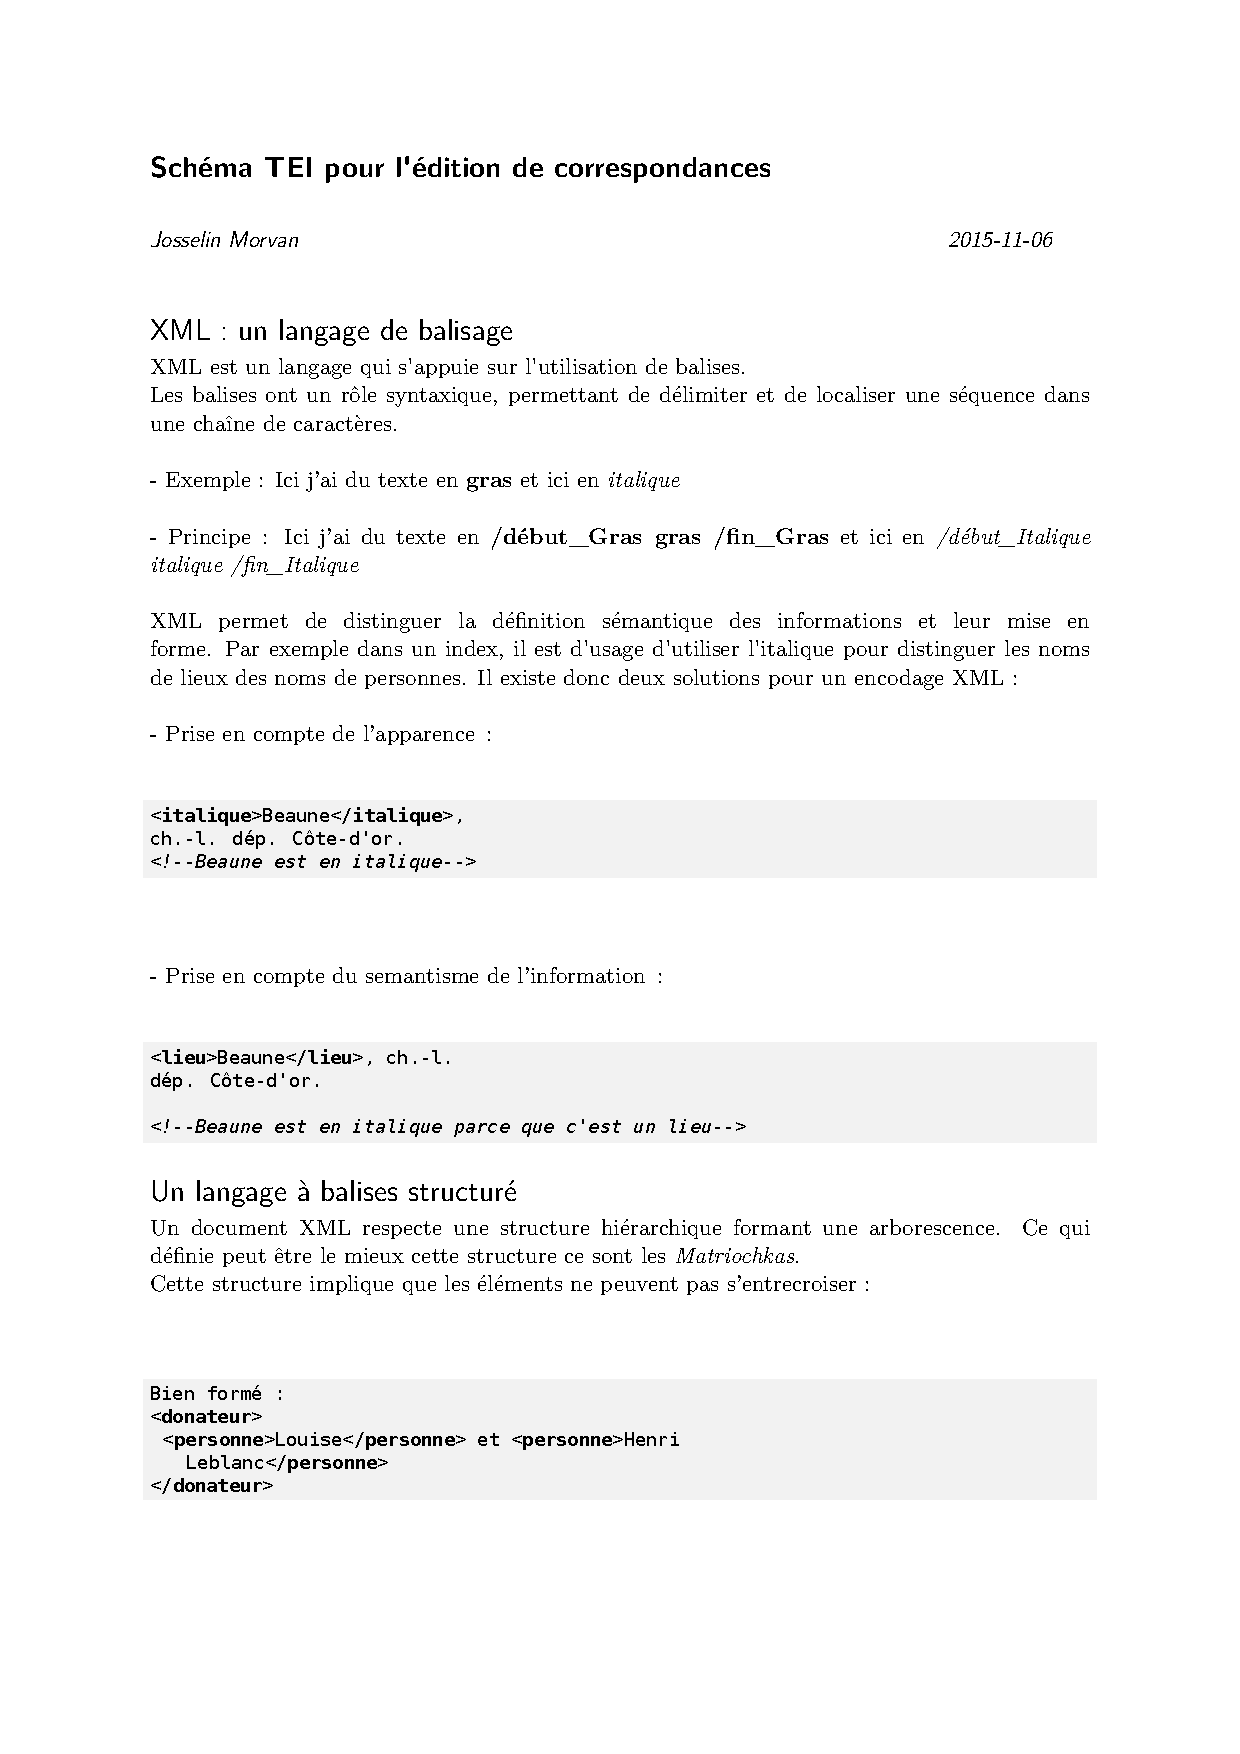
\includepdf[pages=1-21]{documentation_TEI.pdf}
\chapter{Images}
\bigskip


\begin{figure}[!h]
\centering
\begin{center}
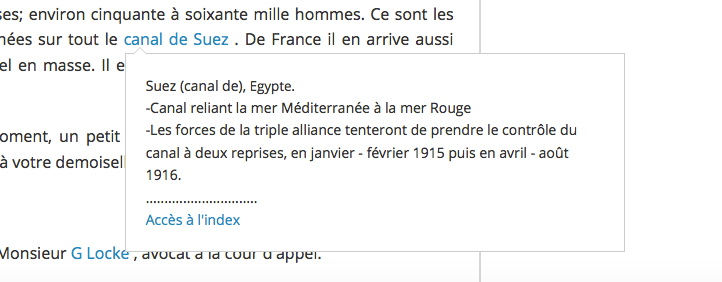
\includegraphics[width=13cm]{1.JPG}
\end{center}
\caption{Exemple de note en survol.}
\end{figure}


\begin{figure}[!h]
\centering
\begin{center}
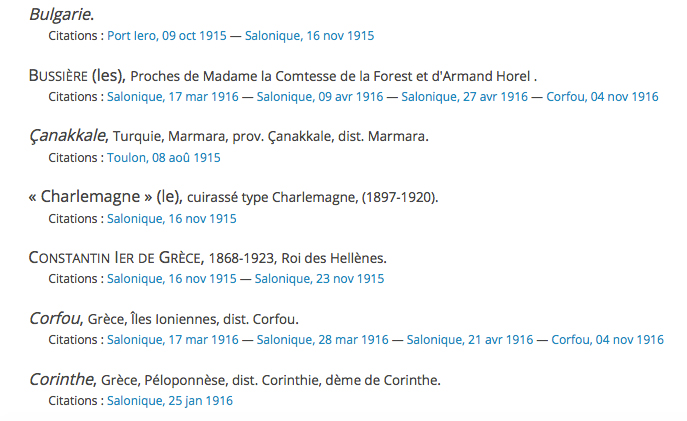
\includegraphics[width=10cm]{2.JPG}
\end{center}
\caption{Exemple d'une partie de l'index.}
\end{figure}


\begin{figure}[!h]
\centering
\begin{center}
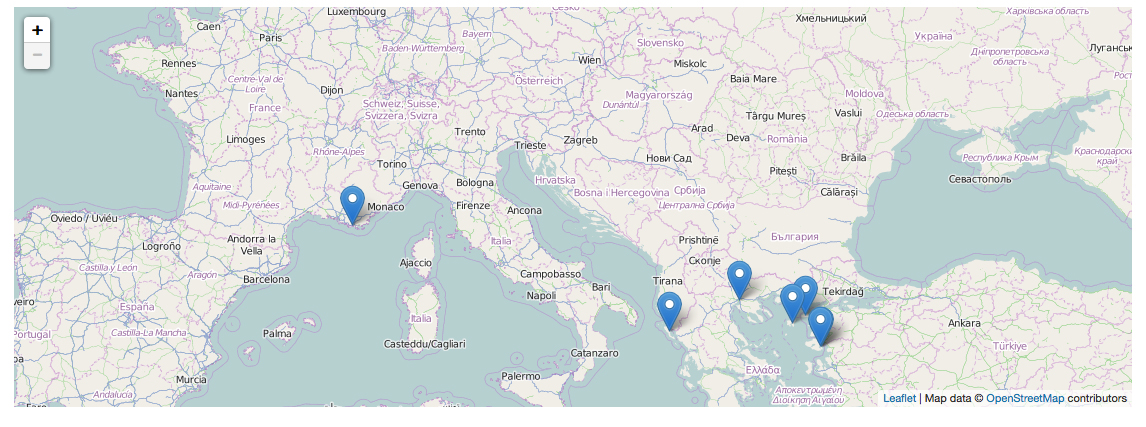
\includegraphics[width=15cm]{4.JPG}
\end{center}
\caption{Cartographie.}
\end{figure}

\begin{figure}[!h]
\centering
\begin{center}
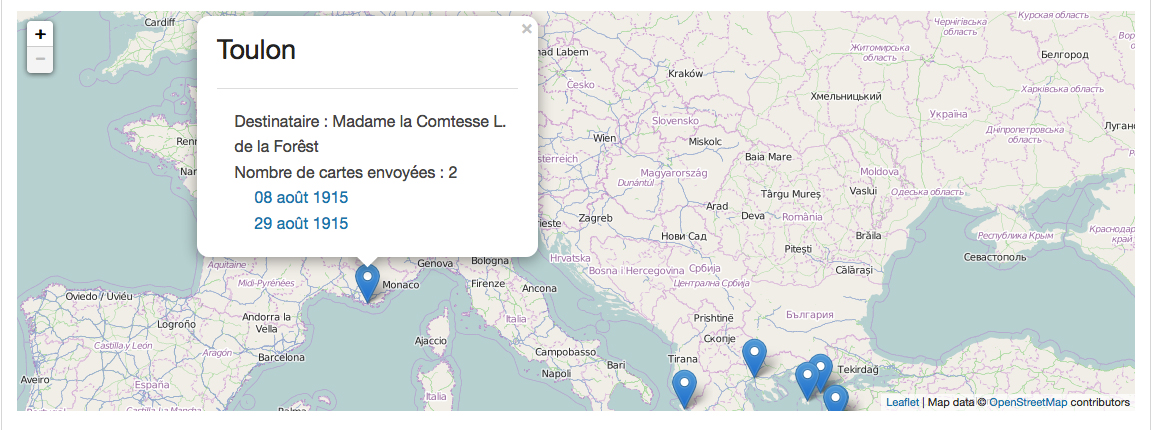
\includegraphics[width=15cm]{5.JPG}
\end{center}
\caption{Cartographie.}
\end{figure}


\begin{figure}[!h]
\centering
\begin{center}
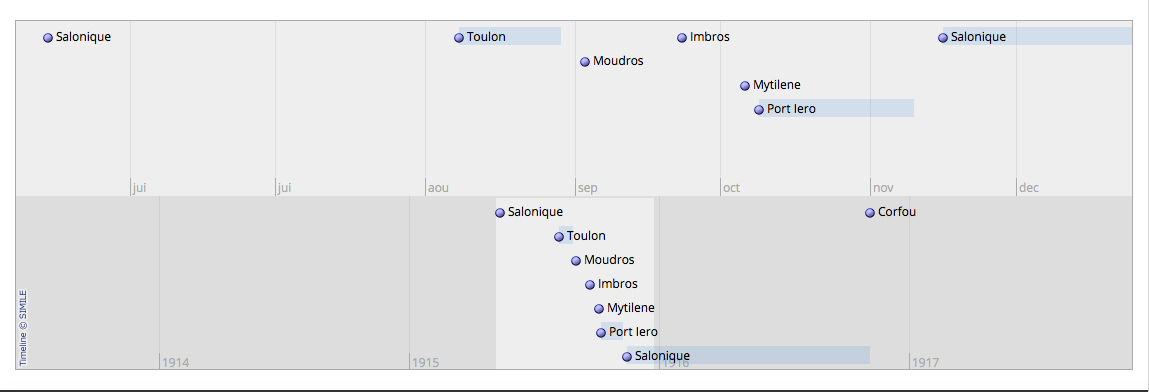
\includegraphics[width=15cm]{3.JPG}
\end{center}
\caption{Frise chronologique.}
\end{figure}

\begin{figure}[!h]
\centering
\begin{center}
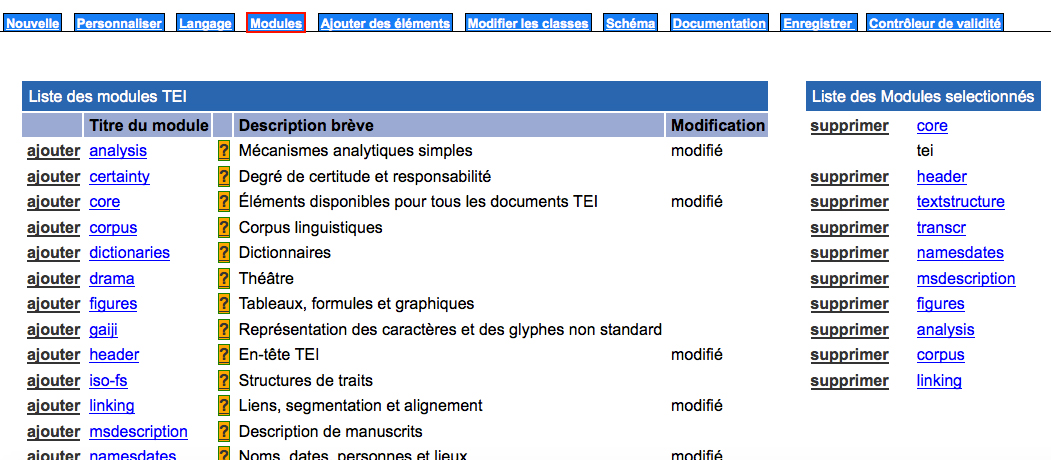
\includegraphics[width=16cm]{8.JPG}
\end{center}
\caption{Roma 2}
\end{figure}

\begin{figure}[!h]
\centering
\begin{center}
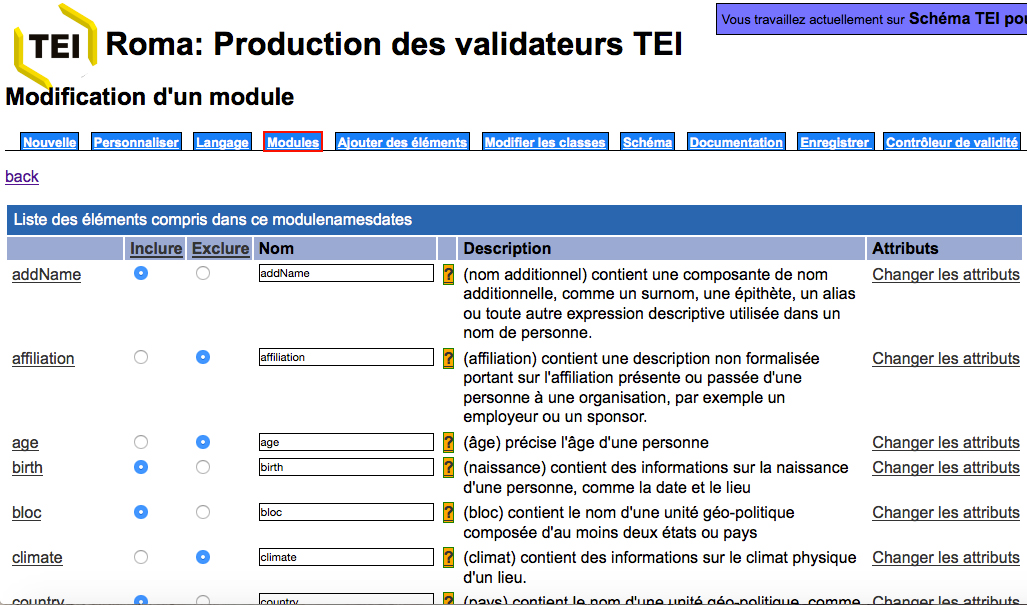
\includegraphics[width=16cm]{6.JPG}
\end{center}
\caption{Roma 1}
\end{figure}





\backmatter

\listoffigures
\tableofcontents

\end{document}
